\only<1>{
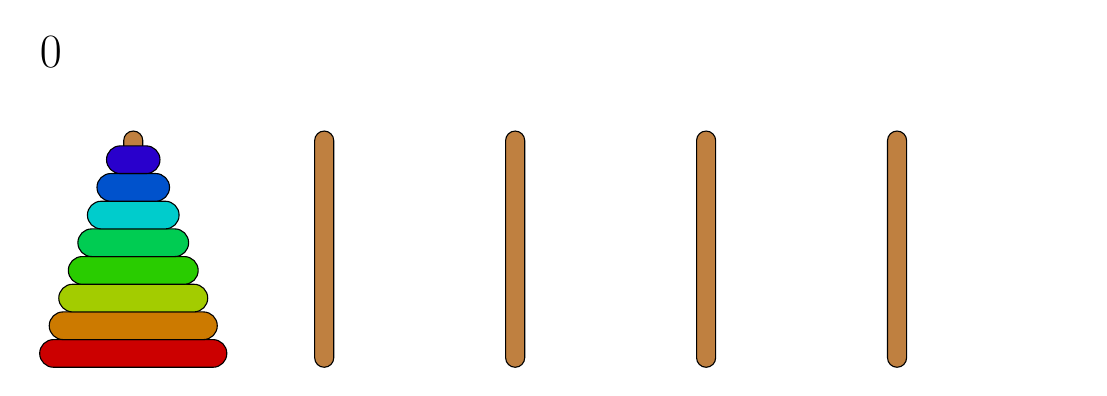
\begin{tikzpicture}
\pgfmathsetlengthmacro\diskheight{10};
\pgfmathsetmacro\k{5};
\pgfmathsetlengthmacro\step{\textwidth/\k};
\node[opacity = 1] at (1.5,4) {\LARGE 0};
\draw[color = white] (\step/2,0) -- (\textwidth+\step,0);
\foreach \n in {1,...,\k} \draw [fill = brown, draw = black, rounded corners = \step/20] (\step*\n,0) rectangle (\step*\n+\step/10,3.0);
\definecolor{mycolor}{rgb:hsb}{0.00,1,0.8}
\draw [fill = mycolor, draw = black, rounded corners = \diskheight/2] (\step*1+\step/20-\step*0.49,\diskheight*0) rectangle (\step*1+\step/20+\step*0.49,\diskheight*1);
\definecolor{mycolor}{rgb:hsb}{0.10,1,0.8}
\draw [fill = mycolor, draw = black, rounded corners = \diskheight/2] (\step*1+\step/20-\step*0.44,\diskheight*1) rectangle (\step*1+\step/20+\step*0.44,\diskheight*2);
\definecolor{mycolor}{rgb:hsb}{0.20,1,0.8}
\draw [fill = mycolor, draw = black, rounded corners = \diskheight/2] (\step*1+\step/20-\step*0.39,\diskheight*2) rectangle (\step*1+\step/20+\step*0.39,\diskheight*3);
\definecolor{mycolor}{rgb:hsb}{0.30,1,0.8}
\draw [fill = mycolor, draw = black, rounded corners = \diskheight/2] (\step*1+\step/20-\step*0.33999999999999997,\diskheight*3) rectangle (\step*1+\step/20+\step*0.33999999999999997,\diskheight*4);
\definecolor{mycolor}{rgb:hsb}{0.40,1,0.8}
\draw [fill = mycolor, draw = black, rounded corners = \diskheight/2] (\step*1+\step/20-\step*0.29,\diskheight*4) rectangle (\step*1+\step/20+\step*0.29,\diskheight*5);
\definecolor{mycolor}{rgb:hsb}{0.50,1,0.8}
\draw [fill = mycolor, draw = black, rounded corners = \diskheight/2] (\step*1+\step/20-\step*0.24,\diskheight*5) rectangle (\step*1+\step/20+\step*0.24,\diskheight*6);
\definecolor{mycolor}{rgb:hsb}{0.60,1,0.8}
\draw [fill = mycolor, draw = black, rounded corners = \diskheight/2] (\step*1+\step/20-\step*0.18999999999999995,\diskheight*6) rectangle (\step*1+\step/20+\step*0.18999999999999995,\diskheight*7);
\definecolor{mycolor}{rgb:hsb}{0.70,1,0.8}
\draw [fill = mycolor, draw = black, rounded corners = \diskheight/2] (\step*1+\step/20-\step*0.13999999999999996,\diskheight*7) rectangle (\step*1+\step/20+\step*0.13999999999999996,\diskheight*8);
\end{tikzpicture}
}
\only<2>{
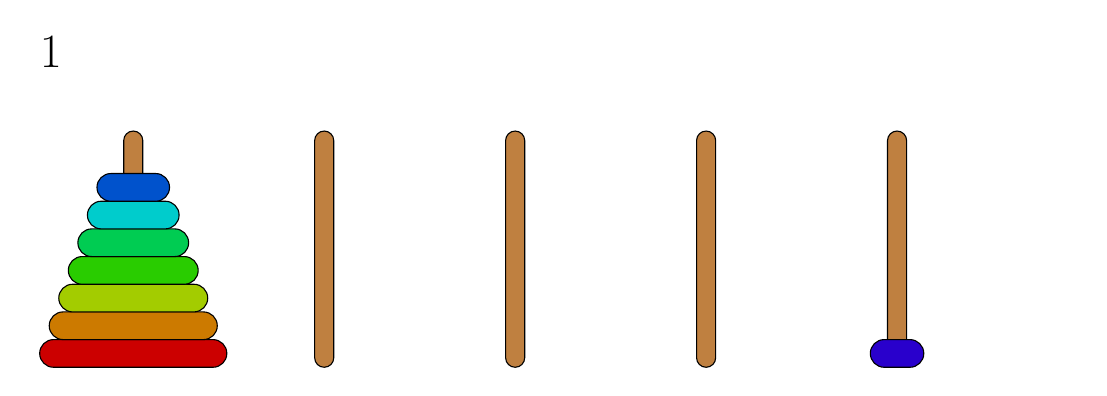
\begin{tikzpicture}
\pgfmathsetlengthmacro\diskheight{10};
\pgfmathsetmacro\k{5};
\pgfmathsetlengthmacro\step{\textwidth/\k};
\node[opacity = 1] at (1.5,4) {\LARGE 1};
\draw[color = white] (\step/2,0) -- (\textwidth+\step,0);
\foreach \n in {1,...,\k} \draw [fill = brown, draw = black, rounded corners = \step/20] (\step*\n,0) rectangle (\step*\n+\step/10,3.0);
\definecolor{mycolor}{rgb:hsb}{0.00,1,0.8}
\draw [fill = mycolor, draw = black, rounded corners = \diskheight/2] (\step*1+\step/20-\step*0.49,\diskheight*0) rectangle (\step*1+\step/20+\step*0.49,\diskheight*1);
\definecolor{mycolor}{rgb:hsb}{0.10,1,0.8}
\draw [fill = mycolor, draw = black, rounded corners = \diskheight/2] (\step*1+\step/20-\step*0.44,\diskheight*1) rectangle (\step*1+\step/20+\step*0.44,\diskheight*2);
\definecolor{mycolor}{rgb:hsb}{0.20,1,0.8}
\draw [fill = mycolor, draw = black, rounded corners = \diskheight/2] (\step*1+\step/20-\step*0.39,\diskheight*2) rectangle (\step*1+\step/20+\step*0.39,\diskheight*3);
\definecolor{mycolor}{rgb:hsb}{0.30,1,0.8}
\draw [fill = mycolor, draw = black, rounded corners = \diskheight/2] (\step*1+\step/20-\step*0.33999999999999997,\diskheight*3) rectangle (\step*1+\step/20+\step*0.33999999999999997,\diskheight*4);
\definecolor{mycolor}{rgb:hsb}{0.40,1,0.8}
\draw [fill = mycolor, draw = black, rounded corners = \diskheight/2] (\step*1+\step/20-\step*0.29,\diskheight*4) rectangle (\step*1+\step/20+\step*0.29,\diskheight*5);
\definecolor{mycolor}{rgb:hsb}{0.50,1,0.8}
\draw [fill = mycolor, draw = black, rounded corners = \diskheight/2] (\step*1+\step/20-\step*0.24,\diskheight*5) rectangle (\step*1+\step/20+\step*0.24,\diskheight*6);
\definecolor{mycolor}{rgb:hsb}{0.60,1,0.8}
\draw [fill = mycolor, draw = black, rounded corners = \diskheight/2] (\step*1+\step/20-\step*0.18999999999999995,\diskheight*6) rectangle (\step*1+\step/20+\step*0.18999999999999995,\diskheight*7);
\definecolor{mycolor}{rgb:hsb}{0.70,1,0.8}
\draw [fill = mycolor, draw = black, rounded corners = \diskheight/2] (\step*5+\step/20-\step*0.13999999999999996,\diskheight*0) rectangle (\step*5+\step/20+\step*0.13999999999999996,\diskheight*1);
\end{tikzpicture}
}
\only<3>{
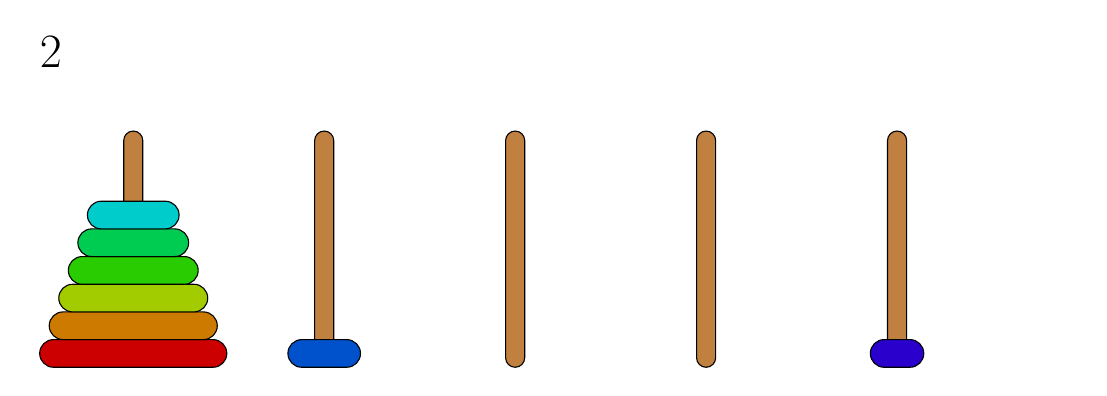
\begin{tikzpicture}
\pgfmathsetlengthmacro\diskheight{10};
\pgfmathsetmacro\k{5};
\pgfmathsetlengthmacro\step{\textwidth/\k};
\node[opacity = 1] at (1.5,4) {\LARGE 2};
\draw[color = white] (\step/2,0) -- (\textwidth+\step,0);
\foreach \n in {1,...,\k} \draw [fill = brown, draw = black, rounded corners = \step/20] (\step*\n,0) rectangle (\step*\n+\step/10,3.0);
\definecolor{mycolor}{rgb:hsb}{0.00,1,0.8}
\draw [fill = mycolor, draw = black, rounded corners = \diskheight/2] (\step*1+\step/20-\step*0.49,\diskheight*0) rectangle (\step*1+\step/20+\step*0.49,\diskheight*1);
\definecolor{mycolor}{rgb:hsb}{0.10,1,0.8}
\draw [fill = mycolor, draw = black, rounded corners = \diskheight/2] (\step*1+\step/20-\step*0.44,\diskheight*1) rectangle (\step*1+\step/20+\step*0.44,\diskheight*2);
\definecolor{mycolor}{rgb:hsb}{0.20,1,0.8}
\draw [fill = mycolor, draw = black, rounded corners = \diskheight/2] (\step*1+\step/20-\step*0.39,\diskheight*2) rectangle (\step*1+\step/20+\step*0.39,\diskheight*3);
\definecolor{mycolor}{rgb:hsb}{0.30,1,0.8}
\draw [fill = mycolor, draw = black, rounded corners = \diskheight/2] (\step*1+\step/20-\step*0.33999999999999997,\diskheight*3) rectangle (\step*1+\step/20+\step*0.33999999999999997,\diskheight*4);
\definecolor{mycolor}{rgb:hsb}{0.40,1,0.8}
\draw [fill = mycolor, draw = black, rounded corners = \diskheight/2] (\step*1+\step/20-\step*0.29,\diskheight*4) rectangle (\step*1+\step/20+\step*0.29,\diskheight*5);
\definecolor{mycolor}{rgb:hsb}{0.50,1,0.8}
\draw [fill = mycolor, draw = black, rounded corners = \diskheight/2] (\step*1+\step/20-\step*0.24,\diskheight*5) rectangle (\step*1+\step/20+\step*0.24,\diskheight*6);
\definecolor{mycolor}{rgb:hsb}{0.60,1,0.8}
\draw [fill = mycolor, draw = black, rounded corners = \diskheight/2] (\step*2+\step/20-\step*0.18999999999999995,\diskheight*0) rectangle (\step*2+\step/20+\step*0.18999999999999995,\diskheight*1);
\definecolor{mycolor}{rgb:hsb}{0.70,1,0.8}
\draw [fill = mycolor, draw = black, rounded corners = \diskheight/2] (\step*5+\step/20-\step*0.13999999999999996,\diskheight*0) rectangle (\step*5+\step/20+\step*0.13999999999999996,\diskheight*1);
\end{tikzpicture}
}
\only<4>{
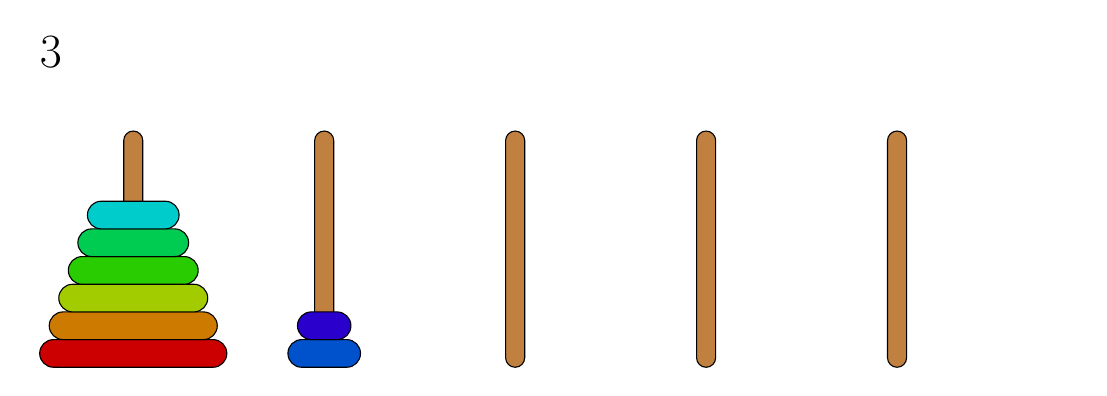
\begin{tikzpicture}
\pgfmathsetlengthmacro\diskheight{10};
\pgfmathsetmacro\k{5};
\pgfmathsetlengthmacro\step{\textwidth/\k};
\node[opacity = 1] at (1.5,4) {\LARGE 3};
\draw[color = white] (\step/2,0) -- (\textwidth+\step,0);
\foreach \n in {1,...,\k} \draw [fill = brown, draw = black, rounded corners = \step/20] (\step*\n,0) rectangle (\step*\n+\step/10,3.0);
\definecolor{mycolor}{rgb:hsb}{0.00,1,0.8}
\draw [fill = mycolor, draw = black, rounded corners = \diskheight/2] (\step*1+\step/20-\step*0.49,\diskheight*0) rectangle (\step*1+\step/20+\step*0.49,\diskheight*1);
\definecolor{mycolor}{rgb:hsb}{0.10,1,0.8}
\draw [fill = mycolor, draw = black, rounded corners = \diskheight/2] (\step*1+\step/20-\step*0.44,\diskheight*1) rectangle (\step*1+\step/20+\step*0.44,\diskheight*2);
\definecolor{mycolor}{rgb:hsb}{0.20,1,0.8}
\draw [fill = mycolor, draw = black, rounded corners = \diskheight/2] (\step*1+\step/20-\step*0.39,\diskheight*2) rectangle (\step*1+\step/20+\step*0.39,\diskheight*3);
\definecolor{mycolor}{rgb:hsb}{0.30,1,0.8}
\draw [fill = mycolor, draw = black, rounded corners = \diskheight/2] (\step*1+\step/20-\step*0.33999999999999997,\diskheight*3) rectangle (\step*1+\step/20+\step*0.33999999999999997,\diskheight*4);
\definecolor{mycolor}{rgb:hsb}{0.40,1,0.8}
\draw [fill = mycolor, draw = black, rounded corners = \diskheight/2] (\step*1+\step/20-\step*0.29,\diskheight*4) rectangle (\step*1+\step/20+\step*0.29,\diskheight*5);
\definecolor{mycolor}{rgb:hsb}{0.50,1,0.8}
\draw [fill = mycolor, draw = black, rounded corners = \diskheight/2] (\step*1+\step/20-\step*0.24,\diskheight*5) rectangle (\step*1+\step/20+\step*0.24,\diskheight*6);
\definecolor{mycolor}{rgb:hsb}{0.60,1,0.8}
\draw [fill = mycolor, draw = black, rounded corners = \diskheight/2] (\step*2+\step/20-\step*0.18999999999999995,\diskheight*0) rectangle (\step*2+\step/20+\step*0.18999999999999995,\diskheight*1);
\definecolor{mycolor}{rgb:hsb}{0.70,1,0.8}
\draw [fill = mycolor, draw = black, rounded corners = \diskheight/2] (\step*2+\step/20-\step*0.13999999999999996,\diskheight*1) rectangle (\step*2+\step/20+\step*0.13999999999999996,\diskheight*2);
\end{tikzpicture}
}
\only<5>{
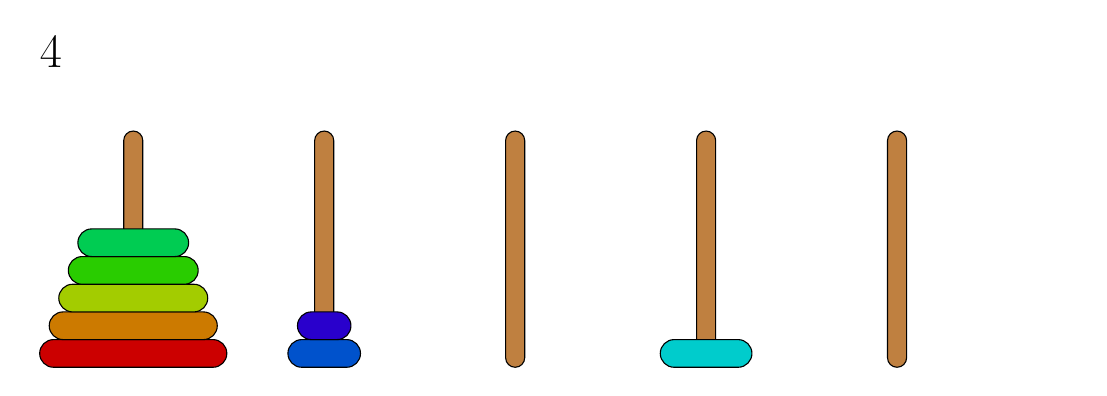
\begin{tikzpicture}
\pgfmathsetlengthmacro\diskheight{10};
\pgfmathsetmacro\k{5};
\pgfmathsetlengthmacro\step{\textwidth/\k};
\node[opacity = 1] at (1.5,4) {\LARGE 4};
\draw[color = white] (\step/2,0) -- (\textwidth+\step,0);
\foreach \n in {1,...,\k} \draw [fill = brown, draw = black, rounded corners = \step/20] (\step*\n,0) rectangle (\step*\n+\step/10,3.0);
\definecolor{mycolor}{rgb:hsb}{0.00,1,0.8}
\draw [fill = mycolor, draw = black, rounded corners = \diskheight/2] (\step*1+\step/20-\step*0.49,\diskheight*0) rectangle (\step*1+\step/20+\step*0.49,\diskheight*1);
\definecolor{mycolor}{rgb:hsb}{0.10,1,0.8}
\draw [fill = mycolor, draw = black, rounded corners = \diskheight/2] (\step*1+\step/20-\step*0.44,\diskheight*1) rectangle (\step*1+\step/20+\step*0.44,\diskheight*2);
\definecolor{mycolor}{rgb:hsb}{0.20,1,0.8}
\draw [fill = mycolor, draw = black, rounded corners = \diskheight/2] (\step*1+\step/20-\step*0.39,\diskheight*2) rectangle (\step*1+\step/20+\step*0.39,\diskheight*3);
\definecolor{mycolor}{rgb:hsb}{0.30,1,0.8}
\draw [fill = mycolor, draw = black, rounded corners = \diskheight/2] (\step*1+\step/20-\step*0.33999999999999997,\diskheight*3) rectangle (\step*1+\step/20+\step*0.33999999999999997,\diskheight*4);
\definecolor{mycolor}{rgb:hsb}{0.40,1,0.8}
\draw [fill = mycolor, draw = black, rounded corners = \diskheight/2] (\step*1+\step/20-\step*0.29,\diskheight*4) rectangle (\step*1+\step/20+\step*0.29,\diskheight*5);
\definecolor{mycolor}{rgb:hsb}{0.60,1,0.8}
\draw [fill = mycolor, draw = black, rounded corners = \diskheight/2] (\step*2+\step/20-\step*0.18999999999999995,\diskheight*0) rectangle (\step*2+\step/20+\step*0.18999999999999995,\diskheight*1);
\definecolor{mycolor}{rgb:hsb}{0.70,1,0.8}
\draw [fill = mycolor, draw = black, rounded corners = \diskheight/2] (\step*2+\step/20-\step*0.13999999999999996,\diskheight*1) rectangle (\step*2+\step/20+\step*0.13999999999999996,\diskheight*2);
\definecolor{mycolor}{rgb:hsb}{0.50,1,0.8}
\draw [fill = mycolor, draw = black, rounded corners = \diskheight/2] (\step*4+\step/20-\step*0.24,\diskheight*0) rectangle (\step*4+\step/20+\step*0.24,\diskheight*1);
\end{tikzpicture}
}
\only<6>{
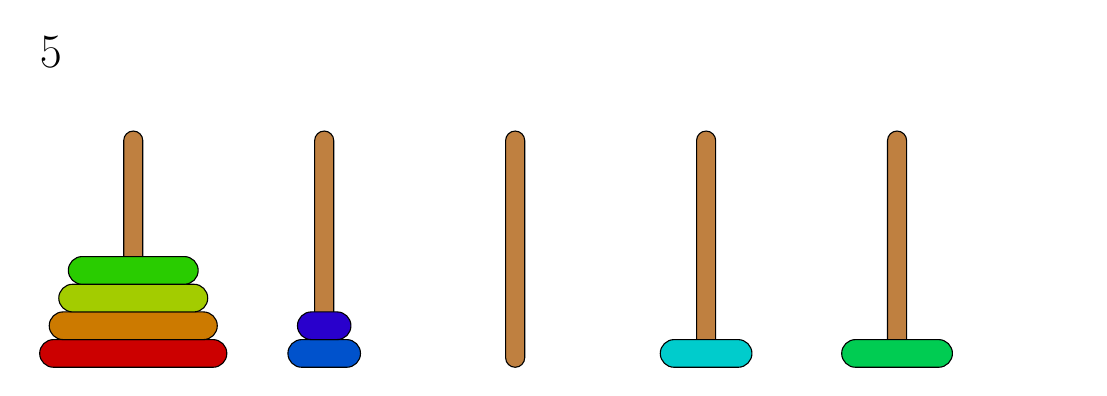
\begin{tikzpicture}
\pgfmathsetlengthmacro\diskheight{10};
\pgfmathsetmacro\k{5};
\pgfmathsetlengthmacro\step{\textwidth/\k};
\node[opacity = 1] at (1.5,4) {\LARGE 5};
\draw[color = white] (\step/2,0) -- (\textwidth+\step,0);
\foreach \n in {1,...,\k} \draw [fill = brown, draw = black, rounded corners = \step/20] (\step*\n,0) rectangle (\step*\n+\step/10,3.0);
\definecolor{mycolor}{rgb:hsb}{0.00,1,0.8}
\draw [fill = mycolor, draw = black, rounded corners = \diskheight/2] (\step*1+\step/20-\step*0.49,\diskheight*0) rectangle (\step*1+\step/20+\step*0.49,\diskheight*1);
\definecolor{mycolor}{rgb:hsb}{0.10,1,0.8}
\draw [fill = mycolor, draw = black, rounded corners = \diskheight/2] (\step*1+\step/20-\step*0.44,\diskheight*1) rectangle (\step*1+\step/20+\step*0.44,\diskheight*2);
\definecolor{mycolor}{rgb:hsb}{0.20,1,0.8}
\draw [fill = mycolor, draw = black, rounded corners = \diskheight/2] (\step*1+\step/20-\step*0.39,\diskheight*2) rectangle (\step*1+\step/20+\step*0.39,\diskheight*3);
\definecolor{mycolor}{rgb:hsb}{0.30,1,0.8}
\draw [fill = mycolor, draw = black, rounded corners = \diskheight/2] (\step*1+\step/20-\step*0.33999999999999997,\diskheight*3) rectangle (\step*1+\step/20+\step*0.33999999999999997,\diskheight*4);
\definecolor{mycolor}{rgb:hsb}{0.60,1,0.8}
\draw [fill = mycolor, draw = black, rounded corners = \diskheight/2] (\step*2+\step/20-\step*0.18999999999999995,\diskheight*0) rectangle (\step*2+\step/20+\step*0.18999999999999995,\diskheight*1);
\definecolor{mycolor}{rgb:hsb}{0.70,1,0.8}
\draw [fill = mycolor, draw = black, rounded corners = \diskheight/2] (\step*2+\step/20-\step*0.13999999999999996,\diskheight*1) rectangle (\step*2+\step/20+\step*0.13999999999999996,\diskheight*2);
\definecolor{mycolor}{rgb:hsb}{0.50,1,0.8}
\draw [fill = mycolor, draw = black, rounded corners = \diskheight/2] (\step*4+\step/20-\step*0.24,\diskheight*0) rectangle (\step*4+\step/20+\step*0.24,\diskheight*1);
\definecolor{mycolor}{rgb:hsb}{0.40,1,0.8}
\draw [fill = mycolor, draw = black, rounded corners = \diskheight/2] (\step*5+\step/20-\step*0.29,\diskheight*0) rectangle (\step*5+\step/20+\step*0.29,\diskheight*1);
\end{tikzpicture}
}
\only<7>{
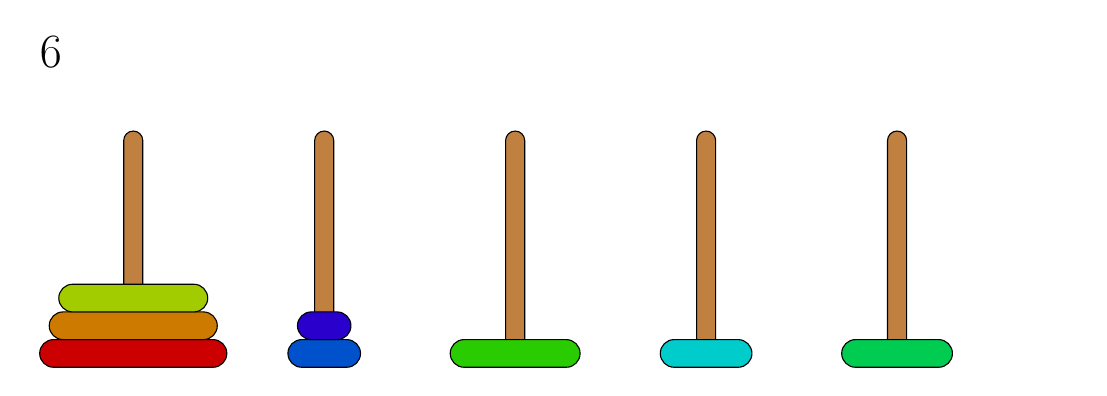
\begin{tikzpicture}
\pgfmathsetlengthmacro\diskheight{10};
\pgfmathsetmacro\k{5};
\pgfmathsetlengthmacro\step{\textwidth/\k};
\node[opacity = 1] at (1.5,4) {\LARGE 6};
\draw[color = white] (\step/2,0) -- (\textwidth+\step,0);
\foreach \n in {1,...,\k} \draw [fill = brown, draw = black, rounded corners = \step/20] (\step*\n,0) rectangle (\step*\n+\step/10,3.0);
\definecolor{mycolor}{rgb:hsb}{0.00,1,0.8}
\draw [fill = mycolor, draw = black, rounded corners = \diskheight/2] (\step*1+\step/20-\step*0.49,\diskheight*0) rectangle (\step*1+\step/20+\step*0.49,\diskheight*1);
\definecolor{mycolor}{rgb:hsb}{0.10,1,0.8}
\draw [fill = mycolor, draw = black, rounded corners = \diskheight/2] (\step*1+\step/20-\step*0.44,\diskheight*1) rectangle (\step*1+\step/20+\step*0.44,\diskheight*2);
\definecolor{mycolor}{rgb:hsb}{0.20,1,0.8}
\draw [fill = mycolor, draw = black, rounded corners = \diskheight/2] (\step*1+\step/20-\step*0.39,\diskheight*2) rectangle (\step*1+\step/20+\step*0.39,\diskheight*3);
\definecolor{mycolor}{rgb:hsb}{0.60,1,0.8}
\draw [fill = mycolor, draw = black, rounded corners = \diskheight/2] (\step*2+\step/20-\step*0.18999999999999995,\diskheight*0) rectangle (\step*2+\step/20+\step*0.18999999999999995,\diskheight*1);
\definecolor{mycolor}{rgb:hsb}{0.70,1,0.8}
\draw [fill = mycolor, draw = black, rounded corners = \diskheight/2] (\step*2+\step/20-\step*0.13999999999999996,\diskheight*1) rectangle (\step*2+\step/20+\step*0.13999999999999996,\diskheight*2);
\definecolor{mycolor}{rgb:hsb}{0.30,1,0.8}
\draw [fill = mycolor, draw = black, rounded corners = \diskheight/2] (\step*3+\step/20-\step*0.33999999999999997,\diskheight*0) rectangle (\step*3+\step/20+\step*0.33999999999999997,\diskheight*1);
\definecolor{mycolor}{rgb:hsb}{0.50,1,0.8}
\draw [fill = mycolor, draw = black, rounded corners = \diskheight/2] (\step*4+\step/20-\step*0.24,\diskheight*0) rectangle (\step*4+\step/20+\step*0.24,\diskheight*1);
\definecolor{mycolor}{rgb:hsb}{0.40,1,0.8}
\draw [fill = mycolor, draw = black, rounded corners = \diskheight/2] (\step*5+\step/20-\step*0.29,\diskheight*0) rectangle (\step*5+\step/20+\step*0.29,\diskheight*1);
\end{tikzpicture}
}
\only<8>{
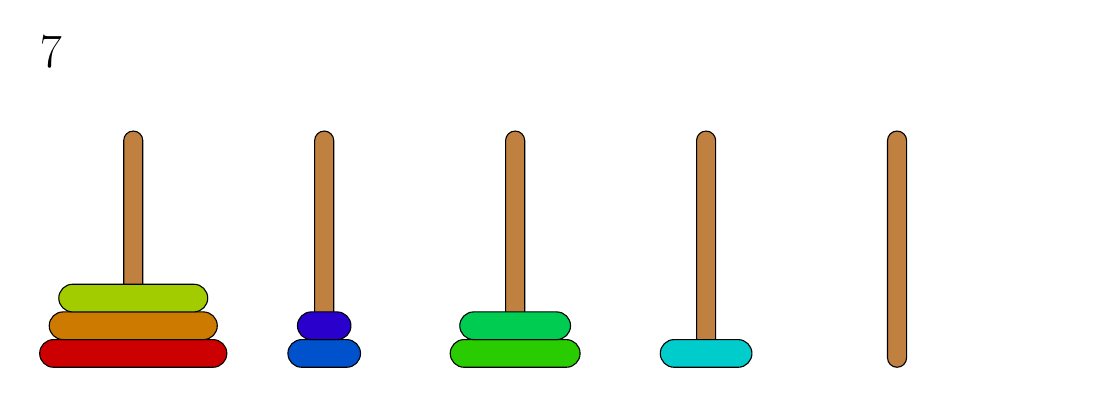
\begin{tikzpicture}
\pgfmathsetlengthmacro\diskheight{10};
\pgfmathsetmacro\k{5};
\pgfmathsetlengthmacro\step{\textwidth/\k};
\node[opacity = 1] at (1.5,4) {\LARGE 7};
\draw[color = white] (\step/2,0) -- (\textwidth+\step,0);
\foreach \n in {1,...,\k} \draw [fill = brown, draw = black, rounded corners = \step/20] (\step*\n,0) rectangle (\step*\n+\step/10,3.0);
\definecolor{mycolor}{rgb:hsb}{0.00,1,0.8}
\draw [fill = mycolor, draw = black, rounded corners = \diskheight/2] (\step*1+\step/20-\step*0.49,\diskheight*0) rectangle (\step*1+\step/20+\step*0.49,\diskheight*1);
\definecolor{mycolor}{rgb:hsb}{0.10,1,0.8}
\draw [fill = mycolor, draw = black, rounded corners = \diskheight/2] (\step*1+\step/20-\step*0.44,\diskheight*1) rectangle (\step*1+\step/20+\step*0.44,\diskheight*2);
\definecolor{mycolor}{rgb:hsb}{0.20,1,0.8}
\draw [fill = mycolor, draw = black, rounded corners = \diskheight/2] (\step*1+\step/20-\step*0.39,\diskheight*2) rectangle (\step*1+\step/20+\step*0.39,\diskheight*3);
\definecolor{mycolor}{rgb:hsb}{0.60,1,0.8}
\draw [fill = mycolor, draw = black, rounded corners = \diskheight/2] (\step*2+\step/20-\step*0.18999999999999995,\diskheight*0) rectangle (\step*2+\step/20+\step*0.18999999999999995,\diskheight*1);
\definecolor{mycolor}{rgb:hsb}{0.70,1,0.8}
\draw [fill = mycolor, draw = black, rounded corners = \diskheight/2] (\step*2+\step/20-\step*0.13999999999999996,\diskheight*1) rectangle (\step*2+\step/20+\step*0.13999999999999996,\diskheight*2);
\definecolor{mycolor}{rgb:hsb}{0.30,1,0.8}
\draw [fill = mycolor, draw = black, rounded corners = \diskheight/2] (\step*3+\step/20-\step*0.33999999999999997,\diskheight*0) rectangle (\step*3+\step/20+\step*0.33999999999999997,\diskheight*1);
\definecolor{mycolor}{rgb:hsb}{0.40,1,0.8}
\draw [fill = mycolor, draw = black, rounded corners = \diskheight/2] (\step*3+\step/20-\step*0.29,\diskheight*1) rectangle (\step*3+\step/20+\step*0.29,\diskheight*2);
\definecolor{mycolor}{rgb:hsb}{0.50,1,0.8}
\draw [fill = mycolor, draw = black, rounded corners = \diskheight/2] (\step*4+\step/20-\step*0.24,\diskheight*0) rectangle (\step*4+\step/20+\step*0.24,\diskheight*1);
\end{tikzpicture}
}
\only<9>{
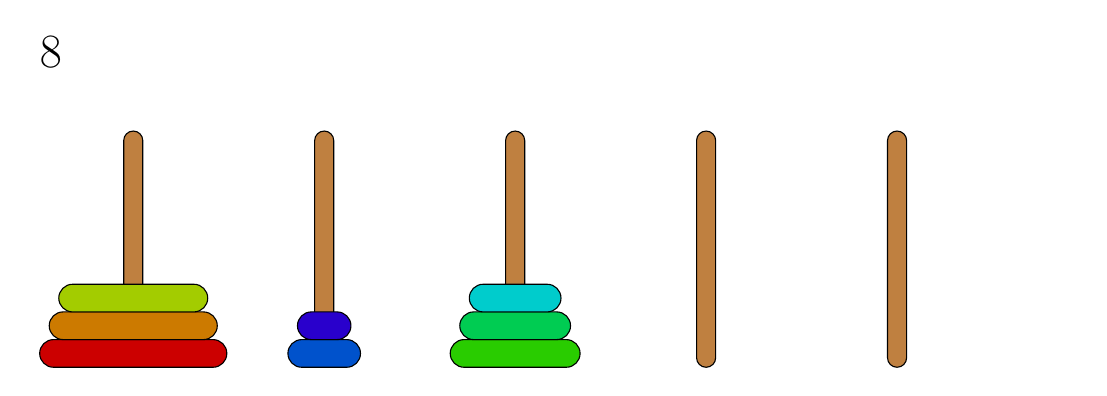
\begin{tikzpicture}
\pgfmathsetlengthmacro\diskheight{10};
\pgfmathsetmacro\k{5};
\pgfmathsetlengthmacro\step{\textwidth/\k};
\node[opacity = 1] at (1.5,4) {\LARGE 8};
\draw[color = white] (\step/2,0) -- (\textwidth+\step,0);
\foreach \n in {1,...,\k} \draw [fill = brown, draw = black, rounded corners = \step/20] (\step*\n,0) rectangle (\step*\n+\step/10,3.0);
\definecolor{mycolor}{rgb:hsb}{0.00,1,0.8}
\draw [fill = mycolor, draw = black, rounded corners = \diskheight/2] (\step*1+\step/20-\step*0.49,\diskheight*0) rectangle (\step*1+\step/20+\step*0.49,\diskheight*1);
\definecolor{mycolor}{rgb:hsb}{0.10,1,0.8}
\draw [fill = mycolor, draw = black, rounded corners = \diskheight/2] (\step*1+\step/20-\step*0.44,\diskheight*1) rectangle (\step*1+\step/20+\step*0.44,\diskheight*2);
\definecolor{mycolor}{rgb:hsb}{0.20,1,0.8}
\draw [fill = mycolor, draw = black, rounded corners = \diskheight/2] (\step*1+\step/20-\step*0.39,\diskheight*2) rectangle (\step*1+\step/20+\step*0.39,\diskheight*3);
\definecolor{mycolor}{rgb:hsb}{0.60,1,0.8}
\draw [fill = mycolor, draw = black, rounded corners = \diskheight/2] (\step*2+\step/20-\step*0.18999999999999995,\diskheight*0) rectangle (\step*2+\step/20+\step*0.18999999999999995,\diskheight*1);
\definecolor{mycolor}{rgb:hsb}{0.70,1,0.8}
\draw [fill = mycolor, draw = black, rounded corners = \diskheight/2] (\step*2+\step/20-\step*0.13999999999999996,\diskheight*1) rectangle (\step*2+\step/20+\step*0.13999999999999996,\diskheight*2);
\definecolor{mycolor}{rgb:hsb}{0.30,1,0.8}
\draw [fill = mycolor, draw = black, rounded corners = \diskheight/2] (\step*3+\step/20-\step*0.33999999999999997,\diskheight*0) rectangle (\step*3+\step/20+\step*0.33999999999999997,\diskheight*1);
\definecolor{mycolor}{rgb:hsb}{0.40,1,0.8}
\draw [fill = mycolor, draw = black, rounded corners = \diskheight/2] (\step*3+\step/20-\step*0.29,\diskheight*1) rectangle (\step*3+\step/20+\step*0.29,\diskheight*2);
\definecolor{mycolor}{rgb:hsb}{0.50,1,0.8}
\draw [fill = mycolor, draw = black, rounded corners = \diskheight/2] (\step*3+\step/20-\step*0.24,\diskheight*2) rectangle (\step*3+\step/20+\step*0.24,\diskheight*3);
\end{tikzpicture}
}
\only<10>{
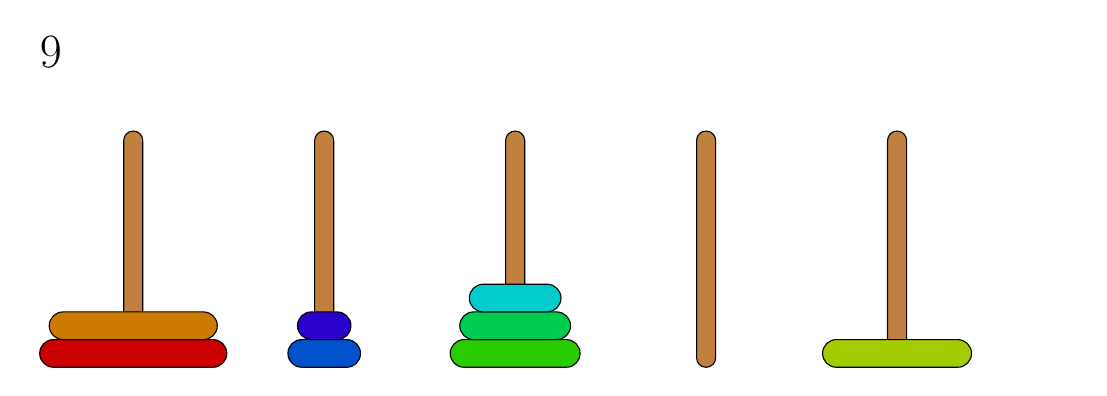
\begin{tikzpicture}
\pgfmathsetlengthmacro\diskheight{10};
\pgfmathsetmacro\k{5};
\pgfmathsetlengthmacro\step{\textwidth/\k};
\node[opacity = 1] at (1.5,4) {\LARGE 9};
\draw[color = white] (\step/2,0) -- (\textwidth+\step,0);
\foreach \n in {1,...,\k} \draw [fill = brown, draw = black, rounded corners = \step/20] (\step*\n,0) rectangle (\step*\n+\step/10,3.0);
\definecolor{mycolor}{rgb:hsb}{0.00,1,0.8}
\draw [fill = mycolor, draw = black, rounded corners = \diskheight/2] (\step*1+\step/20-\step*0.49,\diskheight*0) rectangle (\step*1+\step/20+\step*0.49,\diskheight*1);
\definecolor{mycolor}{rgb:hsb}{0.10,1,0.8}
\draw [fill = mycolor, draw = black, rounded corners = \diskheight/2] (\step*1+\step/20-\step*0.44,\diskheight*1) rectangle (\step*1+\step/20+\step*0.44,\diskheight*2);
\definecolor{mycolor}{rgb:hsb}{0.60,1,0.8}
\draw [fill = mycolor, draw = black, rounded corners = \diskheight/2] (\step*2+\step/20-\step*0.18999999999999995,\diskheight*0) rectangle (\step*2+\step/20+\step*0.18999999999999995,\diskheight*1);
\definecolor{mycolor}{rgb:hsb}{0.70,1,0.8}
\draw [fill = mycolor, draw = black, rounded corners = \diskheight/2] (\step*2+\step/20-\step*0.13999999999999996,\diskheight*1) rectangle (\step*2+\step/20+\step*0.13999999999999996,\diskheight*2);
\definecolor{mycolor}{rgb:hsb}{0.30,1,0.8}
\draw [fill = mycolor, draw = black, rounded corners = \diskheight/2] (\step*3+\step/20-\step*0.33999999999999997,\diskheight*0) rectangle (\step*3+\step/20+\step*0.33999999999999997,\diskheight*1);
\definecolor{mycolor}{rgb:hsb}{0.40,1,0.8}
\draw [fill = mycolor, draw = black, rounded corners = \diskheight/2] (\step*3+\step/20-\step*0.29,\diskheight*1) rectangle (\step*3+\step/20+\step*0.29,\diskheight*2);
\definecolor{mycolor}{rgb:hsb}{0.50,1,0.8}
\draw [fill = mycolor, draw = black, rounded corners = \diskheight/2] (\step*3+\step/20-\step*0.24,\diskheight*2) rectangle (\step*3+\step/20+\step*0.24,\diskheight*3);
\definecolor{mycolor}{rgb:hsb}{0.20,1,0.8}
\draw [fill = mycolor, draw = black, rounded corners = \diskheight/2] (\step*5+\step/20-\step*0.39,\diskheight*0) rectangle (\step*5+\step/20+\step*0.39,\diskheight*1);
\end{tikzpicture}
}
\only<11>{
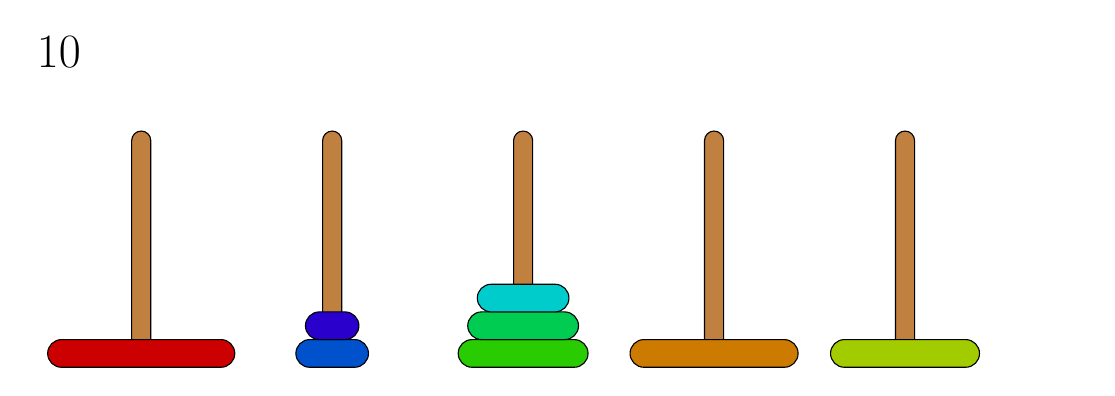
\begin{tikzpicture}
\pgfmathsetlengthmacro\diskheight{10};
\pgfmathsetmacro\k{5};
\pgfmathsetlengthmacro\step{\textwidth/\k};
\node[opacity = 1] at (1.5,4) {\LARGE 10};
\draw[color = white] (\step/2,0) -- (\textwidth+\step,0);
\foreach \n in {1,...,\k} \draw [fill = brown, draw = black, rounded corners = \step/20] (\step*\n,0) rectangle (\step*\n+\step/10,3.0);
\definecolor{mycolor}{rgb:hsb}{0.00,1,0.8}
\draw [fill = mycolor, draw = black, rounded corners = \diskheight/2] (\step*1+\step/20-\step*0.49,\diskheight*0) rectangle (\step*1+\step/20+\step*0.49,\diskheight*1);
\definecolor{mycolor}{rgb:hsb}{0.60,1,0.8}
\draw [fill = mycolor, draw = black, rounded corners = \diskheight/2] (\step*2+\step/20-\step*0.18999999999999995,\diskheight*0) rectangle (\step*2+\step/20+\step*0.18999999999999995,\diskheight*1);
\definecolor{mycolor}{rgb:hsb}{0.70,1,0.8}
\draw [fill = mycolor, draw = black, rounded corners = \diskheight/2] (\step*2+\step/20-\step*0.13999999999999996,\diskheight*1) rectangle (\step*2+\step/20+\step*0.13999999999999996,\diskheight*2);
\definecolor{mycolor}{rgb:hsb}{0.30,1,0.8}
\draw [fill = mycolor, draw = black, rounded corners = \diskheight/2] (\step*3+\step/20-\step*0.33999999999999997,\diskheight*0) rectangle (\step*3+\step/20+\step*0.33999999999999997,\diskheight*1);
\definecolor{mycolor}{rgb:hsb}{0.40,1,0.8}
\draw [fill = mycolor, draw = black, rounded corners = \diskheight/2] (\step*3+\step/20-\step*0.29,\diskheight*1) rectangle (\step*3+\step/20+\step*0.29,\diskheight*2);
\definecolor{mycolor}{rgb:hsb}{0.50,1,0.8}
\draw [fill = mycolor, draw = black, rounded corners = \diskheight/2] (\step*3+\step/20-\step*0.24,\diskheight*2) rectangle (\step*3+\step/20+\step*0.24,\diskheight*3);
\definecolor{mycolor}{rgb:hsb}{0.10,1,0.8}
\draw [fill = mycolor, draw = black, rounded corners = \diskheight/2] (\step*4+\step/20-\step*0.44,\diskheight*0) rectangle (\step*4+\step/20+\step*0.44,\diskheight*1);
\definecolor{mycolor}{rgb:hsb}{0.20,1,0.8}
\draw [fill = mycolor, draw = black, rounded corners = \diskheight/2] (\step*5+\step/20-\step*0.39,\diskheight*0) rectangle (\step*5+\step/20+\step*0.39,\diskheight*1);
\end{tikzpicture}
}
\only<12>{
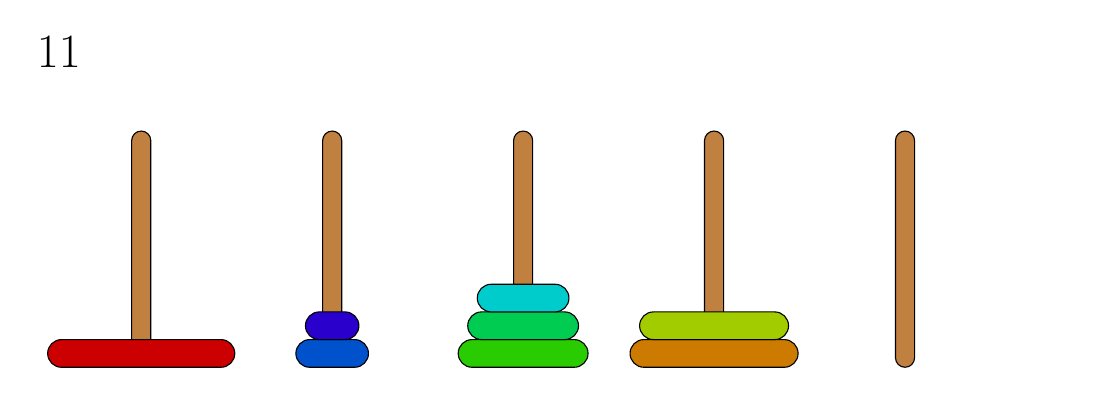
\begin{tikzpicture}
\pgfmathsetlengthmacro\diskheight{10};
\pgfmathsetmacro\k{5};
\pgfmathsetlengthmacro\step{\textwidth/\k};
\node[opacity = 1] at (1.5,4) {\LARGE 11};
\draw[color = white] (\step/2,0) -- (\textwidth+\step,0);
\foreach \n in {1,...,\k} \draw [fill = brown, draw = black, rounded corners = \step/20] (\step*\n,0) rectangle (\step*\n+\step/10,3.0);
\definecolor{mycolor}{rgb:hsb}{0.00,1,0.8}
\draw [fill = mycolor, draw = black, rounded corners = \diskheight/2] (\step*1+\step/20-\step*0.49,\diskheight*0) rectangle (\step*1+\step/20+\step*0.49,\diskheight*1);
\definecolor{mycolor}{rgb:hsb}{0.60,1,0.8}
\draw [fill = mycolor, draw = black, rounded corners = \diskheight/2] (\step*2+\step/20-\step*0.18999999999999995,\diskheight*0) rectangle (\step*2+\step/20+\step*0.18999999999999995,\diskheight*1);
\definecolor{mycolor}{rgb:hsb}{0.70,1,0.8}
\draw [fill = mycolor, draw = black, rounded corners = \diskheight/2] (\step*2+\step/20-\step*0.13999999999999996,\diskheight*1) rectangle (\step*2+\step/20+\step*0.13999999999999996,\diskheight*2);
\definecolor{mycolor}{rgb:hsb}{0.30,1,0.8}
\draw [fill = mycolor, draw = black, rounded corners = \diskheight/2] (\step*3+\step/20-\step*0.33999999999999997,\diskheight*0) rectangle (\step*3+\step/20+\step*0.33999999999999997,\diskheight*1);
\definecolor{mycolor}{rgb:hsb}{0.40,1,0.8}
\draw [fill = mycolor, draw = black, rounded corners = \diskheight/2] (\step*3+\step/20-\step*0.29,\diskheight*1) rectangle (\step*3+\step/20+\step*0.29,\diskheight*2);
\definecolor{mycolor}{rgb:hsb}{0.50,1,0.8}
\draw [fill = mycolor, draw = black, rounded corners = \diskheight/2] (\step*3+\step/20-\step*0.24,\diskheight*2) rectangle (\step*3+\step/20+\step*0.24,\diskheight*3);
\definecolor{mycolor}{rgb:hsb}{0.10,1,0.8}
\draw [fill = mycolor, draw = black, rounded corners = \diskheight/2] (\step*4+\step/20-\step*0.44,\diskheight*0) rectangle (\step*4+\step/20+\step*0.44,\diskheight*1);
\definecolor{mycolor}{rgb:hsb}{0.20,1,0.8}
\draw [fill = mycolor, draw = black, rounded corners = \diskheight/2] (\step*4+\step/20-\step*0.39,\diskheight*1) rectangle (\step*4+\step/20+\step*0.39,\diskheight*2);
\end{tikzpicture}
}
\only<13>{
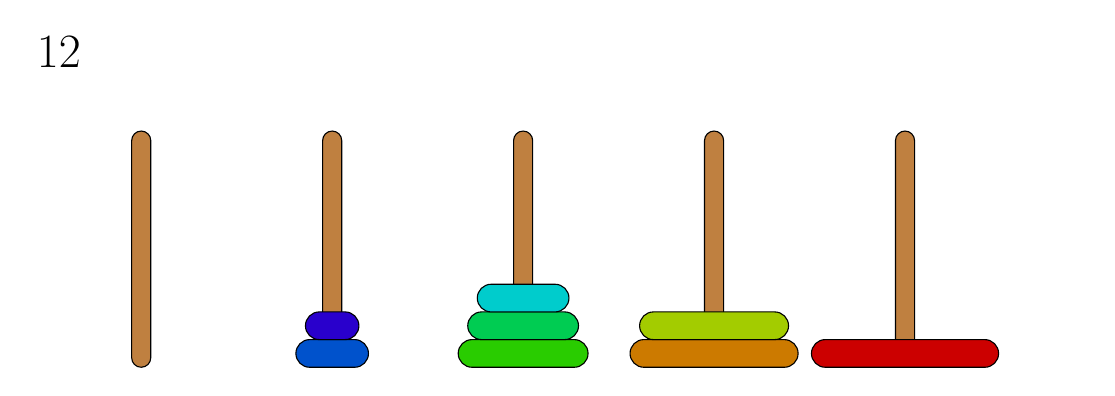
\begin{tikzpicture}
\pgfmathsetlengthmacro\diskheight{10};
\pgfmathsetmacro\k{5};
\pgfmathsetlengthmacro\step{\textwidth/\k};
\node[opacity = 1] at (1.5,4) {\LARGE 12};
\draw[color = white] (\step/2,0) -- (\textwidth+\step,0);
\foreach \n in {1,...,\k} \draw [fill = brown, draw = black, rounded corners = \step/20] (\step*\n,0) rectangle (\step*\n+\step/10,3.0);
\definecolor{mycolor}{rgb:hsb}{0.60,1,0.8}
\draw [fill = mycolor, draw = black, rounded corners = \diskheight/2] (\step*2+\step/20-\step*0.18999999999999995,\diskheight*0) rectangle (\step*2+\step/20+\step*0.18999999999999995,\diskheight*1);
\definecolor{mycolor}{rgb:hsb}{0.70,1,0.8}
\draw [fill = mycolor, draw = black, rounded corners = \diskheight/2] (\step*2+\step/20-\step*0.13999999999999996,\diskheight*1) rectangle (\step*2+\step/20+\step*0.13999999999999996,\diskheight*2);
\definecolor{mycolor}{rgb:hsb}{0.30,1,0.8}
\draw [fill = mycolor, draw = black, rounded corners = \diskheight/2] (\step*3+\step/20-\step*0.33999999999999997,\diskheight*0) rectangle (\step*3+\step/20+\step*0.33999999999999997,\diskheight*1);
\definecolor{mycolor}{rgb:hsb}{0.40,1,0.8}
\draw [fill = mycolor, draw = black, rounded corners = \diskheight/2] (\step*3+\step/20-\step*0.29,\diskheight*1) rectangle (\step*3+\step/20+\step*0.29,\diskheight*2);
\definecolor{mycolor}{rgb:hsb}{0.50,1,0.8}
\draw [fill = mycolor, draw = black, rounded corners = \diskheight/2] (\step*3+\step/20-\step*0.24,\diskheight*2) rectangle (\step*3+\step/20+\step*0.24,\diskheight*3);
\definecolor{mycolor}{rgb:hsb}{0.10,1,0.8}
\draw [fill = mycolor, draw = black, rounded corners = \diskheight/2] (\step*4+\step/20-\step*0.44,\diskheight*0) rectangle (\step*4+\step/20+\step*0.44,\diskheight*1);
\definecolor{mycolor}{rgb:hsb}{0.20,1,0.8}
\draw [fill = mycolor, draw = black, rounded corners = \diskheight/2] (\step*4+\step/20-\step*0.39,\diskheight*1) rectangle (\step*4+\step/20+\step*0.39,\diskheight*2);
\definecolor{mycolor}{rgb:hsb}{0.00,1,0.8}
\draw [fill = mycolor, draw = black, rounded corners = \diskheight/2] (\step*5+\step/20-\step*0.49,\diskheight*0) rectangle (\step*5+\step/20+\step*0.49,\diskheight*1);
\end{tikzpicture}
}
\only<14>{
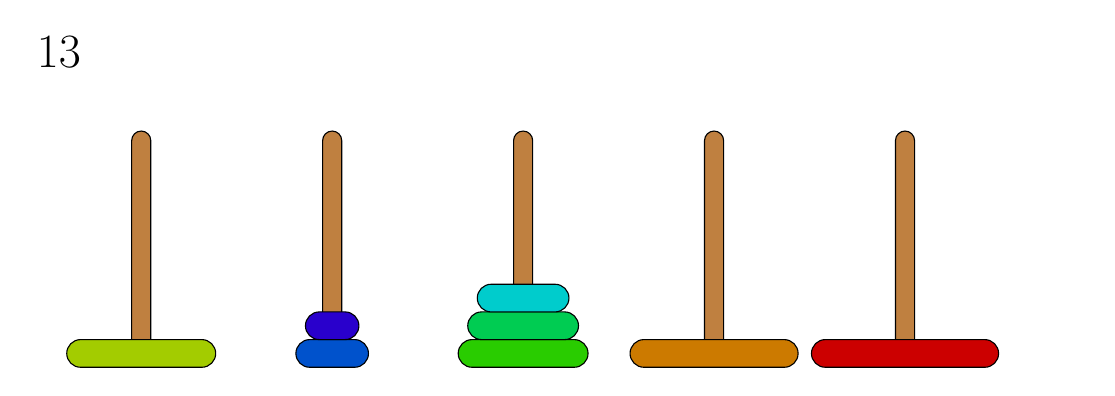
\begin{tikzpicture}
\pgfmathsetlengthmacro\diskheight{10};
\pgfmathsetmacro\k{5};
\pgfmathsetlengthmacro\step{\textwidth/\k};
\node[opacity = 1] at (1.5,4) {\LARGE 13};
\draw[color = white] (\step/2,0) -- (\textwidth+\step,0);
\foreach \n in {1,...,\k} \draw [fill = brown, draw = black, rounded corners = \step/20] (\step*\n,0) rectangle (\step*\n+\step/10,3.0);
\definecolor{mycolor}{rgb:hsb}{0.20,1,0.8}
\draw [fill = mycolor, draw = black, rounded corners = \diskheight/2] (\step*1+\step/20-\step*0.39,\diskheight*0) rectangle (\step*1+\step/20+\step*0.39,\diskheight*1);
\definecolor{mycolor}{rgb:hsb}{0.60,1,0.8}
\draw [fill = mycolor, draw = black, rounded corners = \diskheight/2] (\step*2+\step/20-\step*0.18999999999999995,\diskheight*0) rectangle (\step*2+\step/20+\step*0.18999999999999995,\diskheight*1);
\definecolor{mycolor}{rgb:hsb}{0.70,1,0.8}
\draw [fill = mycolor, draw = black, rounded corners = \diskheight/2] (\step*2+\step/20-\step*0.13999999999999996,\diskheight*1) rectangle (\step*2+\step/20+\step*0.13999999999999996,\diskheight*2);
\definecolor{mycolor}{rgb:hsb}{0.30,1,0.8}
\draw [fill = mycolor, draw = black, rounded corners = \diskheight/2] (\step*3+\step/20-\step*0.33999999999999997,\diskheight*0) rectangle (\step*3+\step/20+\step*0.33999999999999997,\diskheight*1);
\definecolor{mycolor}{rgb:hsb}{0.40,1,0.8}
\draw [fill = mycolor, draw = black, rounded corners = \diskheight/2] (\step*3+\step/20-\step*0.29,\diskheight*1) rectangle (\step*3+\step/20+\step*0.29,\diskheight*2);
\definecolor{mycolor}{rgb:hsb}{0.50,1,0.8}
\draw [fill = mycolor, draw = black, rounded corners = \diskheight/2] (\step*3+\step/20-\step*0.24,\diskheight*2) rectangle (\step*3+\step/20+\step*0.24,\diskheight*3);
\definecolor{mycolor}{rgb:hsb}{0.10,1,0.8}
\draw [fill = mycolor, draw = black, rounded corners = \diskheight/2] (\step*4+\step/20-\step*0.44,\diskheight*0) rectangle (\step*4+\step/20+\step*0.44,\diskheight*1);
\definecolor{mycolor}{rgb:hsb}{0.00,1,0.8}
\draw [fill = mycolor, draw = black, rounded corners = \diskheight/2] (\step*5+\step/20-\step*0.49,\diskheight*0) rectangle (\step*5+\step/20+\step*0.49,\diskheight*1);
\end{tikzpicture}
}
\only<15>{
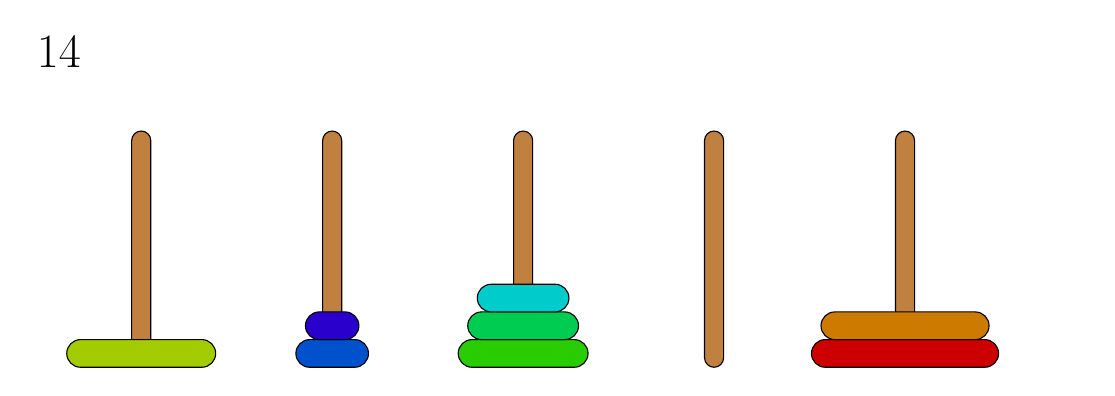
\begin{tikzpicture}
\pgfmathsetlengthmacro\diskheight{10};
\pgfmathsetmacro\k{5};
\pgfmathsetlengthmacro\step{\textwidth/\k};
\node[opacity = 1] at (1.5,4) {\LARGE 14};
\draw[color = white] (\step/2,0) -- (\textwidth+\step,0);
\foreach \n in {1,...,\k} \draw [fill = brown, draw = black, rounded corners = \step/20] (\step*\n,0) rectangle (\step*\n+\step/10,3.0);
\definecolor{mycolor}{rgb:hsb}{0.20,1,0.8}
\draw [fill = mycolor, draw = black, rounded corners = \diskheight/2] (\step*1+\step/20-\step*0.39,\diskheight*0) rectangle (\step*1+\step/20+\step*0.39,\diskheight*1);
\definecolor{mycolor}{rgb:hsb}{0.60,1,0.8}
\draw [fill = mycolor, draw = black, rounded corners = \diskheight/2] (\step*2+\step/20-\step*0.18999999999999995,\diskheight*0) rectangle (\step*2+\step/20+\step*0.18999999999999995,\diskheight*1);
\definecolor{mycolor}{rgb:hsb}{0.70,1,0.8}
\draw [fill = mycolor, draw = black, rounded corners = \diskheight/2] (\step*2+\step/20-\step*0.13999999999999996,\diskheight*1) rectangle (\step*2+\step/20+\step*0.13999999999999996,\diskheight*2);
\definecolor{mycolor}{rgb:hsb}{0.30,1,0.8}
\draw [fill = mycolor, draw = black, rounded corners = \diskheight/2] (\step*3+\step/20-\step*0.33999999999999997,\diskheight*0) rectangle (\step*3+\step/20+\step*0.33999999999999997,\diskheight*1);
\definecolor{mycolor}{rgb:hsb}{0.40,1,0.8}
\draw [fill = mycolor, draw = black, rounded corners = \diskheight/2] (\step*3+\step/20-\step*0.29,\diskheight*1) rectangle (\step*3+\step/20+\step*0.29,\diskheight*2);
\definecolor{mycolor}{rgb:hsb}{0.50,1,0.8}
\draw [fill = mycolor, draw = black, rounded corners = \diskheight/2] (\step*3+\step/20-\step*0.24,\diskheight*2) rectangle (\step*3+\step/20+\step*0.24,\diskheight*3);
\definecolor{mycolor}{rgb:hsb}{0.00,1,0.8}
\draw [fill = mycolor, draw = black, rounded corners = \diskheight/2] (\step*5+\step/20-\step*0.49,\diskheight*0) rectangle (\step*5+\step/20+\step*0.49,\diskheight*1);
\definecolor{mycolor}{rgb:hsb}{0.10,1,0.8}
\draw [fill = mycolor, draw = black, rounded corners = \diskheight/2] (\step*5+\step/20-\step*0.44,\diskheight*1) rectangle (\step*5+\step/20+\step*0.44,\diskheight*2);
\end{tikzpicture}
}
\only<16>{
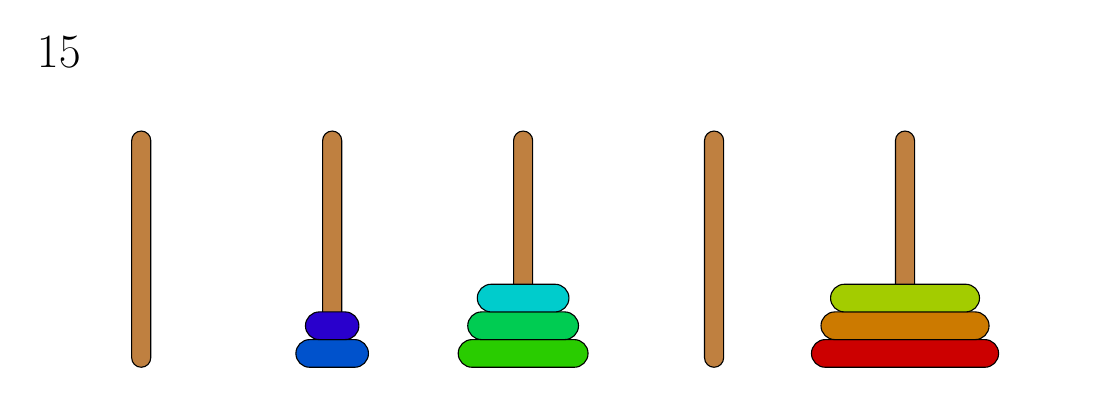
\begin{tikzpicture}
\pgfmathsetlengthmacro\diskheight{10};
\pgfmathsetmacro\k{5};
\pgfmathsetlengthmacro\step{\textwidth/\k};
\node[opacity = 1] at (1.5,4) {\LARGE 15};
\draw[color = white] (\step/2,0) -- (\textwidth+\step,0);
\foreach \n in {1,...,\k} \draw [fill = brown, draw = black, rounded corners = \step/20] (\step*\n,0) rectangle (\step*\n+\step/10,3.0);
\definecolor{mycolor}{rgb:hsb}{0.60,1,0.8}
\draw [fill = mycolor, draw = black, rounded corners = \diskheight/2] (\step*2+\step/20-\step*0.18999999999999995,\diskheight*0) rectangle (\step*2+\step/20+\step*0.18999999999999995,\diskheight*1);
\definecolor{mycolor}{rgb:hsb}{0.70,1,0.8}
\draw [fill = mycolor, draw = black, rounded corners = \diskheight/2] (\step*2+\step/20-\step*0.13999999999999996,\diskheight*1) rectangle (\step*2+\step/20+\step*0.13999999999999996,\diskheight*2);
\definecolor{mycolor}{rgb:hsb}{0.30,1,0.8}
\draw [fill = mycolor, draw = black, rounded corners = \diskheight/2] (\step*3+\step/20-\step*0.33999999999999997,\diskheight*0) rectangle (\step*3+\step/20+\step*0.33999999999999997,\diskheight*1);
\definecolor{mycolor}{rgb:hsb}{0.40,1,0.8}
\draw [fill = mycolor, draw = black, rounded corners = \diskheight/2] (\step*3+\step/20-\step*0.29,\diskheight*1) rectangle (\step*3+\step/20+\step*0.29,\diskheight*2);
\definecolor{mycolor}{rgb:hsb}{0.50,1,0.8}
\draw [fill = mycolor, draw = black, rounded corners = \diskheight/2] (\step*3+\step/20-\step*0.24,\diskheight*2) rectangle (\step*3+\step/20+\step*0.24,\diskheight*3);
\definecolor{mycolor}{rgb:hsb}{0.00,1,0.8}
\draw [fill = mycolor, draw = black, rounded corners = \diskheight/2] (\step*5+\step/20-\step*0.49,\diskheight*0) rectangle (\step*5+\step/20+\step*0.49,\diskheight*1);
\definecolor{mycolor}{rgb:hsb}{0.10,1,0.8}
\draw [fill = mycolor, draw = black, rounded corners = \diskheight/2] (\step*5+\step/20-\step*0.44,\diskheight*1) rectangle (\step*5+\step/20+\step*0.44,\diskheight*2);
\definecolor{mycolor}{rgb:hsb}{0.20,1,0.8}
\draw [fill = mycolor, draw = black, rounded corners = \diskheight/2] (\step*5+\step/20-\step*0.39,\diskheight*2) rectangle (\step*5+\step/20+\step*0.39,\diskheight*3);
\end{tikzpicture}
}
\only<17>{
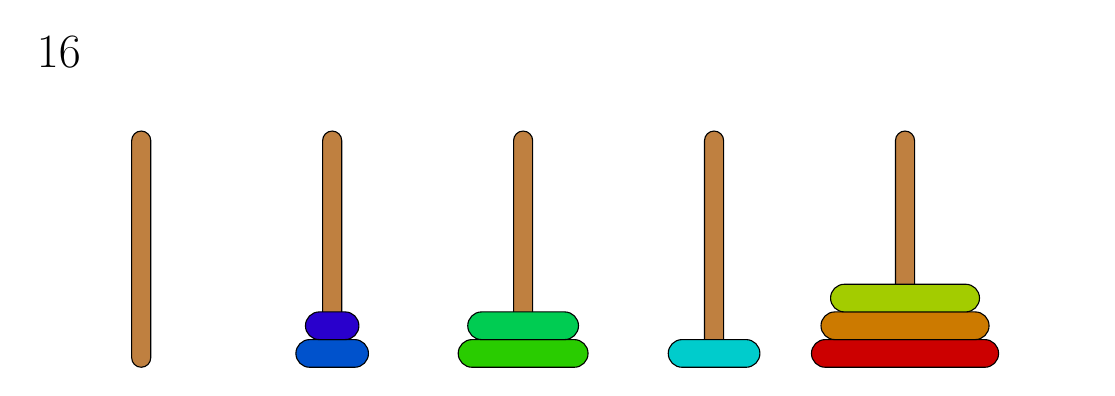
\begin{tikzpicture}
\pgfmathsetlengthmacro\diskheight{10};
\pgfmathsetmacro\k{5};
\pgfmathsetlengthmacro\step{\textwidth/\k};
\node[opacity = 1] at (1.5,4) {\LARGE 16};
\draw[color = white] (\step/2,0) -- (\textwidth+\step,0);
\foreach \n in {1,...,\k} \draw [fill = brown, draw = black, rounded corners = \step/20] (\step*\n,0) rectangle (\step*\n+\step/10,3.0);
\definecolor{mycolor}{rgb:hsb}{0.60,1,0.8}
\draw [fill = mycolor, draw = black, rounded corners = \diskheight/2] (\step*2+\step/20-\step*0.18999999999999995,\diskheight*0) rectangle (\step*2+\step/20+\step*0.18999999999999995,\diskheight*1);
\definecolor{mycolor}{rgb:hsb}{0.70,1,0.8}
\draw [fill = mycolor, draw = black, rounded corners = \diskheight/2] (\step*2+\step/20-\step*0.13999999999999996,\diskheight*1) rectangle (\step*2+\step/20+\step*0.13999999999999996,\diskheight*2);
\definecolor{mycolor}{rgb:hsb}{0.30,1,0.8}
\draw [fill = mycolor, draw = black, rounded corners = \diskheight/2] (\step*3+\step/20-\step*0.33999999999999997,\diskheight*0) rectangle (\step*3+\step/20+\step*0.33999999999999997,\diskheight*1);
\definecolor{mycolor}{rgb:hsb}{0.40,1,0.8}
\draw [fill = mycolor, draw = black, rounded corners = \diskheight/2] (\step*3+\step/20-\step*0.29,\diskheight*1) rectangle (\step*3+\step/20+\step*0.29,\diskheight*2);
\definecolor{mycolor}{rgb:hsb}{0.50,1,0.8}
\draw [fill = mycolor, draw = black, rounded corners = \diskheight/2] (\step*4+\step/20-\step*0.24,\diskheight*0) rectangle (\step*4+\step/20+\step*0.24,\diskheight*1);
\definecolor{mycolor}{rgb:hsb}{0.00,1,0.8}
\draw [fill = mycolor, draw = black, rounded corners = \diskheight/2] (\step*5+\step/20-\step*0.49,\diskheight*0) rectangle (\step*5+\step/20+\step*0.49,\diskheight*1);
\definecolor{mycolor}{rgb:hsb}{0.10,1,0.8}
\draw [fill = mycolor, draw = black, rounded corners = \diskheight/2] (\step*5+\step/20-\step*0.44,\diskheight*1) rectangle (\step*5+\step/20+\step*0.44,\diskheight*2);
\definecolor{mycolor}{rgb:hsb}{0.20,1,0.8}
\draw [fill = mycolor, draw = black, rounded corners = \diskheight/2] (\step*5+\step/20-\step*0.39,\diskheight*2) rectangle (\step*5+\step/20+\step*0.39,\diskheight*3);
\end{tikzpicture}
}
\only<18>{
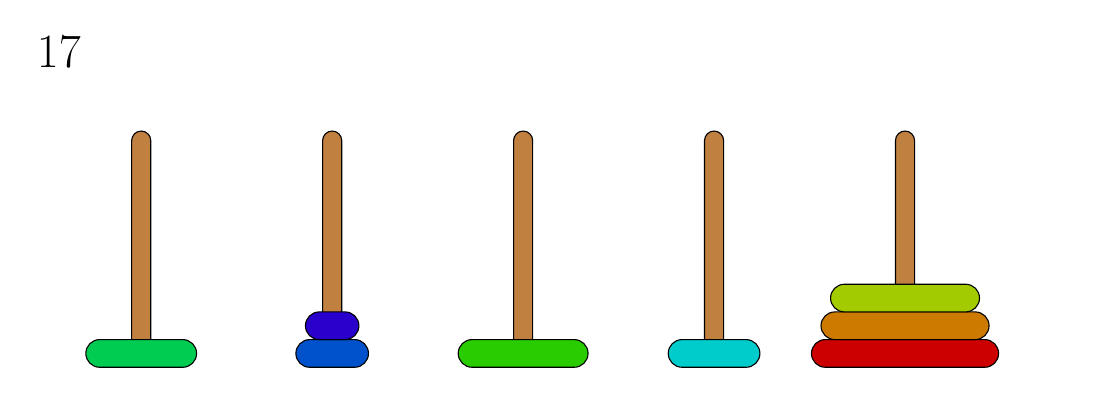
\begin{tikzpicture}
\pgfmathsetlengthmacro\diskheight{10};
\pgfmathsetmacro\k{5};
\pgfmathsetlengthmacro\step{\textwidth/\k};
\node[opacity = 1] at (1.5,4) {\LARGE 17};
\draw[color = white] (\step/2,0) -- (\textwidth+\step,0);
\foreach \n in {1,...,\k} \draw [fill = brown, draw = black, rounded corners = \step/20] (\step*\n,0) rectangle (\step*\n+\step/10,3.0);
\definecolor{mycolor}{rgb:hsb}{0.40,1,0.8}
\draw [fill = mycolor, draw = black, rounded corners = \diskheight/2] (\step*1+\step/20-\step*0.29,\diskheight*0) rectangle (\step*1+\step/20+\step*0.29,\diskheight*1);
\definecolor{mycolor}{rgb:hsb}{0.60,1,0.8}
\draw [fill = mycolor, draw = black, rounded corners = \diskheight/2] (\step*2+\step/20-\step*0.18999999999999995,\diskheight*0) rectangle (\step*2+\step/20+\step*0.18999999999999995,\diskheight*1);
\definecolor{mycolor}{rgb:hsb}{0.70,1,0.8}
\draw [fill = mycolor, draw = black, rounded corners = \diskheight/2] (\step*2+\step/20-\step*0.13999999999999996,\diskheight*1) rectangle (\step*2+\step/20+\step*0.13999999999999996,\diskheight*2);
\definecolor{mycolor}{rgb:hsb}{0.30,1,0.8}
\draw [fill = mycolor, draw = black, rounded corners = \diskheight/2] (\step*3+\step/20-\step*0.33999999999999997,\diskheight*0) rectangle (\step*3+\step/20+\step*0.33999999999999997,\diskheight*1);
\definecolor{mycolor}{rgb:hsb}{0.50,1,0.8}
\draw [fill = mycolor, draw = black, rounded corners = \diskheight/2] (\step*4+\step/20-\step*0.24,\diskheight*0) rectangle (\step*4+\step/20+\step*0.24,\diskheight*1);
\definecolor{mycolor}{rgb:hsb}{0.00,1,0.8}
\draw [fill = mycolor, draw = black, rounded corners = \diskheight/2] (\step*5+\step/20-\step*0.49,\diskheight*0) rectangle (\step*5+\step/20+\step*0.49,\diskheight*1);
\definecolor{mycolor}{rgb:hsb}{0.10,1,0.8}
\draw [fill = mycolor, draw = black, rounded corners = \diskheight/2] (\step*5+\step/20-\step*0.44,\diskheight*1) rectangle (\step*5+\step/20+\step*0.44,\diskheight*2);
\definecolor{mycolor}{rgb:hsb}{0.20,1,0.8}
\draw [fill = mycolor, draw = black, rounded corners = \diskheight/2] (\step*5+\step/20-\step*0.39,\diskheight*2) rectangle (\step*5+\step/20+\step*0.39,\diskheight*3);
\end{tikzpicture}
}
\only<19>{
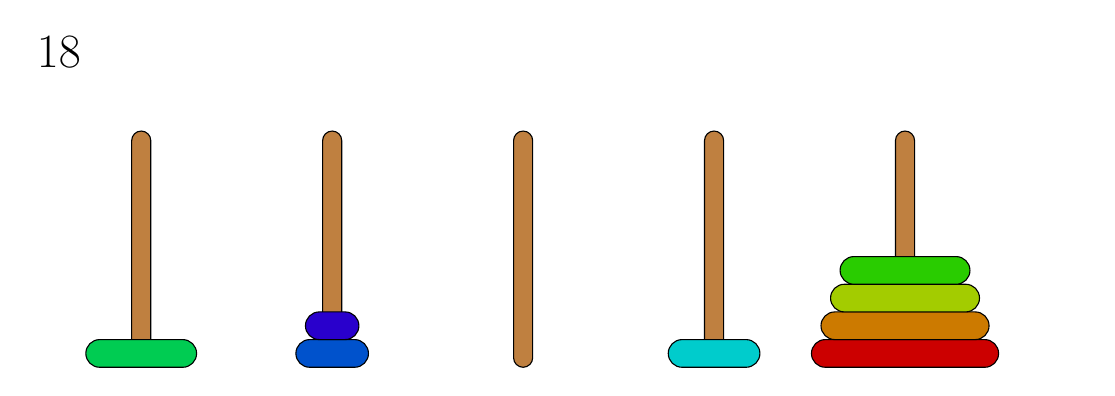
\begin{tikzpicture}
\pgfmathsetlengthmacro\diskheight{10};
\pgfmathsetmacro\k{5};
\pgfmathsetlengthmacro\step{\textwidth/\k};
\node[opacity = 1] at (1.5,4) {\LARGE 18};
\draw[color = white] (\step/2,0) -- (\textwidth+\step,0);
\foreach \n in {1,...,\k} \draw [fill = brown, draw = black, rounded corners = \step/20] (\step*\n,0) rectangle (\step*\n+\step/10,3.0);
\definecolor{mycolor}{rgb:hsb}{0.40,1,0.8}
\draw [fill = mycolor, draw = black, rounded corners = \diskheight/2] (\step*1+\step/20-\step*0.29,\diskheight*0) rectangle (\step*1+\step/20+\step*0.29,\diskheight*1);
\definecolor{mycolor}{rgb:hsb}{0.60,1,0.8}
\draw [fill = mycolor, draw = black, rounded corners = \diskheight/2] (\step*2+\step/20-\step*0.18999999999999995,\diskheight*0) rectangle (\step*2+\step/20+\step*0.18999999999999995,\diskheight*1);
\definecolor{mycolor}{rgb:hsb}{0.70,1,0.8}
\draw [fill = mycolor, draw = black, rounded corners = \diskheight/2] (\step*2+\step/20-\step*0.13999999999999996,\diskheight*1) rectangle (\step*2+\step/20+\step*0.13999999999999996,\diskheight*2);
\definecolor{mycolor}{rgb:hsb}{0.50,1,0.8}
\draw [fill = mycolor, draw = black, rounded corners = \diskheight/2] (\step*4+\step/20-\step*0.24,\diskheight*0) rectangle (\step*4+\step/20+\step*0.24,\diskheight*1);
\definecolor{mycolor}{rgb:hsb}{0.00,1,0.8}
\draw [fill = mycolor, draw = black, rounded corners = \diskheight/2] (\step*5+\step/20-\step*0.49,\diskheight*0) rectangle (\step*5+\step/20+\step*0.49,\diskheight*1);
\definecolor{mycolor}{rgb:hsb}{0.10,1,0.8}
\draw [fill = mycolor, draw = black, rounded corners = \diskheight/2] (\step*5+\step/20-\step*0.44,\diskheight*1) rectangle (\step*5+\step/20+\step*0.44,\diskheight*2);
\definecolor{mycolor}{rgb:hsb}{0.20,1,0.8}
\draw [fill = mycolor, draw = black, rounded corners = \diskheight/2] (\step*5+\step/20-\step*0.39,\diskheight*2) rectangle (\step*5+\step/20+\step*0.39,\diskheight*3);
\definecolor{mycolor}{rgb:hsb}{0.30,1,0.8}
\draw [fill = mycolor, draw = black, rounded corners = \diskheight/2] (\step*5+\step/20-\step*0.33999999999999997,\diskheight*3) rectangle (\step*5+\step/20+\step*0.33999999999999997,\diskheight*4);
\end{tikzpicture}
}
\only<20>{
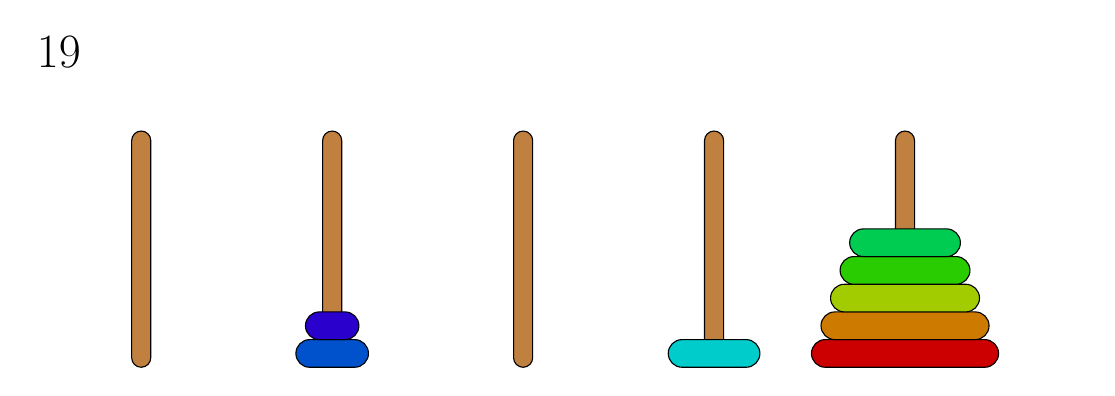
\begin{tikzpicture}
\pgfmathsetlengthmacro\diskheight{10};
\pgfmathsetmacro\k{5};
\pgfmathsetlengthmacro\step{\textwidth/\k};
\node[opacity = 1] at (1.5,4) {\LARGE 19};
\draw[color = white] (\step/2,0) -- (\textwidth+\step,0);
\foreach \n in {1,...,\k} \draw [fill = brown, draw = black, rounded corners = \step/20] (\step*\n,0) rectangle (\step*\n+\step/10,3.0);
\definecolor{mycolor}{rgb:hsb}{0.60,1,0.8}
\draw [fill = mycolor, draw = black, rounded corners = \diskheight/2] (\step*2+\step/20-\step*0.18999999999999995,\diskheight*0) rectangle (\step*2+\step/20+\step*0.18999999999999995,\diskheight*1);
\definecolor{mycolor}{rgb:hsb}{0.70,1,0.8}
\draw [fill = mycolor, draw = black, rounded corners = \diskheight/2] (\step*2+\step/20-\step*0.13999999999999996,\diskheight*1) rectangle (\step*2+\step/20+\step*0.13999999999999996,\diskheight*2);
\definecolor{mycolor}{rgb:hsb}{0.50,1,0.8}
\draw [fill = mycolor, draw = black, rounded corners = \diskheight/2] (\step*4+\step/20-\step*0.24,\diskheight*0) rectangle (\step*4+\step/20+\step*0.24,\diskheight*1);
\definecolor{mycolor}{rgb:hsb}{0.00,1,0.8}
\draw [fill = mycolor, draw = black, rounded corners = \diskheight/2] (\step*5+\step/20-\step*0.49,\diskheight*0) rectangle (\step*5+\step/20+\step*0.49,\diskheight*1);
\definecolor{mycolor}{rgb:hsb}{0.10,1,0.8}
\draw [fill = mycolor, draw = black, rounded corners = \diskheight/2] (\step*5+\step/20-\step*0.44,\diskheight*1) rectangle (\step*5+\step/20+\step*0.44,\diskheight*2);
\definecolor{mycolor}{rgb:hsb}{0.20,1,0.8}
\draw [fill = mycolor, draw = black, rounded corners = \diskheight/2] (\step*5+\step/20-\step*0.39,\diskheight*2) rectangle (\step*5+\step/20+\step*0.39,\diskheight*3);
\definecolor{mycolor}{rgb:hsb}{0.30,1,0.8}
\draw [fill = mycolor, draw = black, rounded corners = \diskheight/2] (\step*5+\step/20-\step*0.33999999999999997,\diskheight*3) rectangle (\step*5+\step/20+\step*0.33999999999999997,\diskheight*4);
\definecolor{mycolor}{rgb:hsb}{0.40,1,0.8}
\draw [fill = mycolor, draw = black, rounded corners = \diskheight/2] (\step*5+\step/20-\step*0.29,\diskheight*4) rectangle (\step*5+\step/20+\step*0.29,\diskheight*5);
\end{tikzpicture}
}
\only<21>{
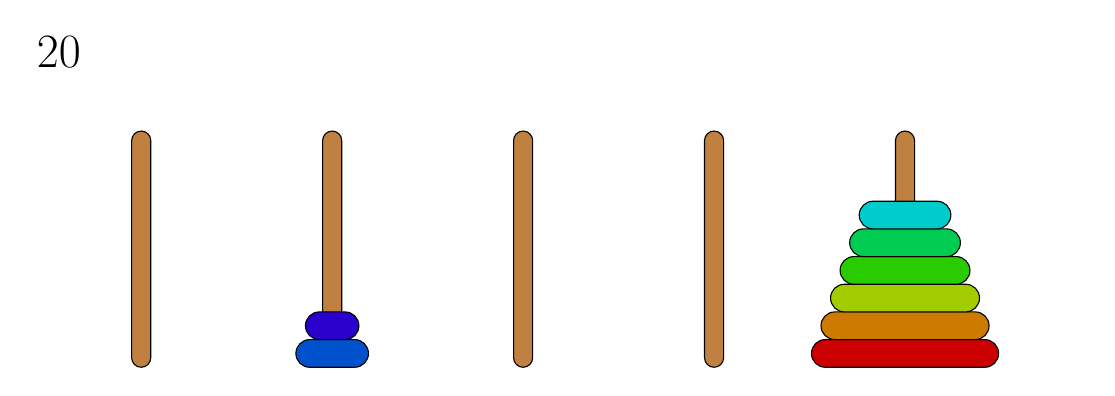
\begin{tikzpicture}
\pgfmathsetlengthmacro\diskheight{10};
\pgfmathsetmacro\k{5};
\pgfmathsetlengthmacro\step{\textwidth/\k};
\node[opacity = 1] at (1.5,4) {\LARGE 20};
\draw[color = white] (\step/2,0) -- (\textwidth+\step,0);
\foreach \n in {1,...,\k} \draw [fill = brown, draw = black, rounded corners = \step/20] (\step*\n,0) rectangle (\step*\n+\step/10,3.0);
\definecolor{mycolor}{rgb:hsb}{0.60,1,0.8}
\draw [fill = mycolor, draw = black, rounded corners = \diskheight/2] (\step*2+\step/20-\step*0.18999999999999995,\diskheight*0) rectangle (\step*2+\step/20+\step*0.18999999999999995,\diskheight*1);
\definecolor{mycolor}{rgb:hsb}{0.70,1,0.8}
\draw [fill = mycolor, draw = black, rounded corners = \diskheight/2] (\step*2+\step/20-\step*0.13999999999999996,\diskheight*1) rectangle (\step*2+\step/20+\step*0.13999999999999996,\diskheight*2);
\definecolor{mycolor}{rgb:hsb}{0.00,1,0.8}
\draw [fill = mycolor, draw = black, rounded corners = \diskheight/2] (\step*5+\step/20-\step*0.49,\diskheight*0) rectangle (\step*5+\step/20+\step*0.49,\diskheight*1);
\definecolor{mycolor}{rgb:hsb}{0.10,1,0.8}
\draw [fill = mycolor, draw = black, rounded corners = \diskheight/2] (\step*5+\step/20-\step*0.44,\diskheight*1) rectangle (\step*5+\step/20+\step*0.44,\diskheight*2);
\definecolor{mycolor}{rgb:hsb}{0.20,1,0.8}
\draw [fill = mycolor, draw = black, rounded corners = \diskheight/2] (\step*5+\step/20-\step*0.39,\diskheight*2) rectangle (\step*5+\step/20+\step*0.39,\diskheight*3);
\definecolor{mycolor}{rgb:hsb}{0.30,1,0.8}
\draw [fill = mycolor, draw = black, rounded corners = \diskheight/2] (\step*5+\step/20-\step*0.33999999999999997,\diskheight*3) rectangle (\step*5+\step/20+\step*0.33999999999999997,\diskheight*4);
\definecolor{mycolor}{rgb:hsb}{0.40,1,0.8}
\draw [fill = mycolor, draw = black, rounded corners = \diskheight/2] (\step*5+\step/20-\step*0.29,\diskheight*4) rectangle (\step*5+\step/20+\step*0.29,\diskheight*5);
\definecolor{mycolor}{rgb:hsb}{0.50,1,0.8}
\draw [fill = mycolor, draw = black, rounded corners = \diskheight/2] (\step*5+\step/20-\step*0.24,\diskheight*5) rectangle (\step*5+\step/20+\step*0.24,\diskheight*6);
\end{tikzpicture}
}
\only<22>{
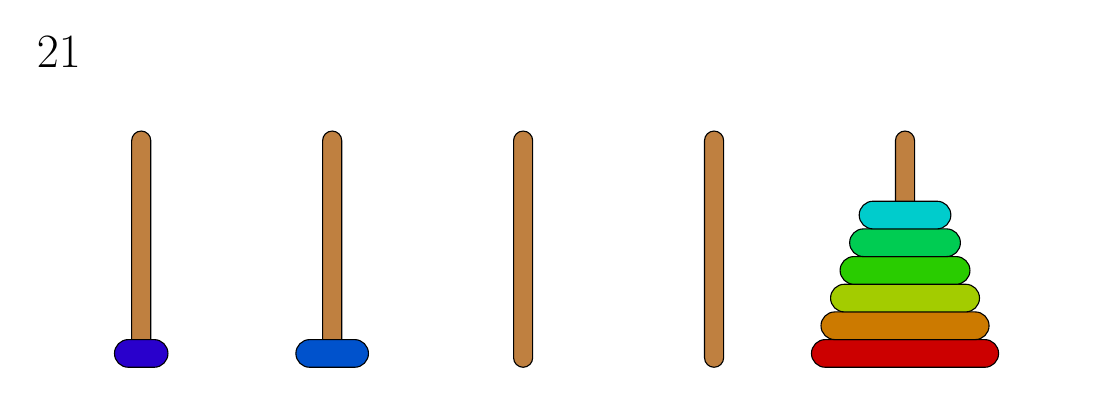
\begin{tikzpicture}
\pgfmathsetlengthmacro\diskheight{10};
\pgfmathsetmacro\k{5};
\pgfmathsetlengthmacro\step{\textwidth/\k};
\node[opacity = 1] at (1.5,4) {\LARGE 21};
\draw[color = white] (\step/2,0) -- (\textwidth+\step,0);
\foreach \n in {1,...,\k} \draw [fill = brown, draw = black, rounded corners = \step/20] (\step*\n,0) rectangle (\step*\n+\step/10,3.0);
\definecolor{mycolor}{rgb:hsb}{0.70,1,0.8}
\draw [fill = mycolor, draw = black, rounded corners = \diskheight/2] (\step*1+\step/20-\step*0.13999999999999996,\diskheight*0) rectangle (\step*1+\step/20+\step*0.13999999999999996,\diskheight*1);
\definecolor{mycolor}{rgb:hsb}{0.60,1,0.8}
\draw [fill = mycolor, draw = black, rounded corners = \diskheight/2] (\step*2+\step/20-\step*0.18999999999999995,\diskheight*0) rectangle (\step*2+\step/20+\step*0.18999999999999995,\diskheight*1);
\definecolor{mycolor}{rgb:hsb}{0.00,1,0.8}
\draw [fill = mycolor, draw = black, rounded corners = \diskheight/2] (\step*5+\step/20-\step*0.49,\diskheight*0) rectangle (\step*5+\step/20+\step*0.49,\diskheight*1);
\definecolor{mycolor}{rgb:hsb}{0.10,1,0.8}
\draw [fill = mycolor, draw = black, rounded corners = \diskheight/2] (\step*5+\step/20-\step*0.44,\diskheight*1) rectangle (\step*5+\step/20+\step*0.44,\diskheight*2);
\definecolor{mycolor}{rgb:hsb}{0.20,1,0.8}
\draw [fill = mycolor, draw = black, rounded corners = \diskheight/2] (\step*5+\step/20-\step*0.39,\diskheight*2) rectangle (\step*5+\step/20+\step*0.39,\diskheight*3);
\definecolor{mycolor}{rgb:hsb}{0.30,1,0.8}
\draw [fill = mycolor, draw = black, rounded corners = \diskheight/2] (\step*5+\step/20-\step*0.33999999999999997,\diskheight*3) rectangle (\step*5+\step/20+\step*0.33999999999999997,\diskheight*4);
\definecolor{mycolor}{rgb:hsb}{0.40,1,0.8}
\draw [fill = mycolor, draw = black, rounded corners = \diskheight/2] (\step*5+\step/20-\step*0.29,\diskheight*4) rectangle (\step*5+\step/20+\step*0.29,\diskheight*5);
\definecolor{mycolor}{rgb:hsb}{0.50,1,0.8}
\draw [fill = mycolor, draw = black, rounded corners = \diskheight/2] (\step*5+\step/20-\step*0.24,\diskheight*5) rectangle (\step*5+\step/20+\step*0.24,\diskheight*6);
\end{tikzpicture}
}
\only<23>{
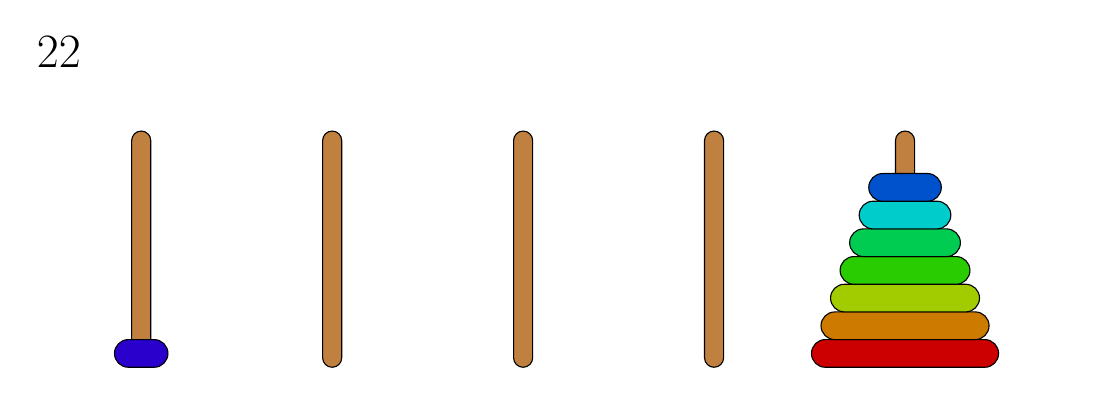
\begin{tikzpicture}
\pgfmathsetlengthmacro\diskheight{10};
\pgfmathsetmacro\k{5};
\pgfmathsetlengthmacro\step{\textwidth/\k};
\node[opacity = 1] at (1.5,4) {\LARGE 22};
\draw[color = white] (\step/2,0) -- (\textwidth+\step,0);
\foreach \n in {1,...,\k} \draw [fill = brown, draw = black, rounded corners = \step/20] (\step*\n,0) rectangle (\step*\n+\step/10,3.0);
\definecolor{mycolor}{rgb:hsb}{0.70,1,0.8}
\draw [fill = mycolor, draw = black, rounded corners = \diskheight/2] (\step*1+\step/20-\step*0.13999999999999996,\diskheight*0) rectangle (\step*1+\step/20+\step*0.13999999999999996,\diskheight*1);
\definecolor{mycolor}{rgb:hsb}{0.00,1,0.8}
\draw [fill = mycolor, draw = black, rounded corners = \diskheight/2] (\step*5+\step/20-\step*0.49,\diskheight*0) rectangle (\step*5+\step/20+\step*0.49,\diskheight*1);
\definecolor{mycolor}{rgb:hsb}{0.10,1,0.8}
\draw [fill = mycolor, draw = black, rounded corners = \diskheight/2] (\step*5+\step/20-\step*0.44,\diskheight*1) rectangle (\step*5+\step/20+\step*0.44,\diskheight*2);
\definecolor{mycolor}{rgb:hsb}{0.20,1,0.8}
\draw [fill = mycolor, draw = black, rounded corners = \diskheight/2] (\step*5+\step/20-\step*0.39,\diskheight*2) rectangle (\step*5+\step/20+\step*0.39,\diskheight*3);
\definecolor{mycolor}{rgb:hsb}{0.30,1,0.8}
\draw [fill = mycolor, draw = black, rounded corners = \diskheight/2] (\step*5+\step/20-\step*0.33999999999999997,\diskheight*3) rectangle (\step*5+\step/20+\step*0.33999999999999997,\diskheight*4);
\definecolor{mycolor}{rgb:hsb}{0.40,1,0.8}
\draw [fill = mycolor, draw = black, rounded corners = \diskheight/2] (\step*5+\step/20-\step*0.29,\diskheight*4) rectangle (\step*5+\step/20+\step*0.29,\diskheight*5);
\definecolor{mycolor}{rgb:hsb}{0.50,1,0.8}
\draw [fill = mycolor, draw = black, rounded corners = \diskheight/2] (\step*5+\step/20-\step*0.24,\diskheight*5) rectangle (\step*5+\step/20+\step*0.24,\diskheight*6);
\definecolor{mycolor}{rgb:hsb}{0.60,1,0.8}
\draw [fill = mycolor, draw = black, rounded corners = \diskheight/2] (\step*5+\step/20-\step*0.18999999999999995,\diskheight*6) rectangle (\step*5+\step/20+\step*0.18999999999999995,\diskheight*7);
\end{tikzpicture}
}
\only<24>{
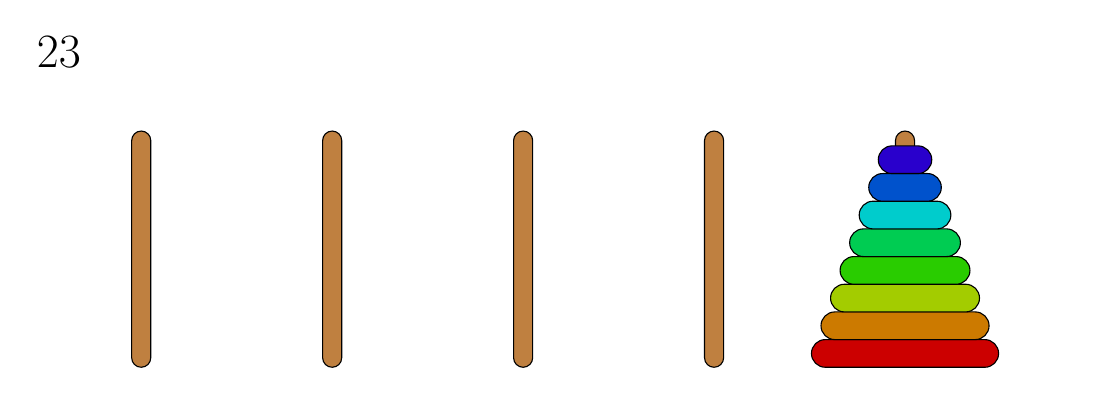
\begin{tikzpicture}
\pgfmathsetlengthmacro\diskheight{10};
\pgfmathsetmacro\k{5};
\pgfmathsetlengthmacro\step{\textwidth/\k};
\node[opacity = 1] at (1.5,4) {\LARGE 23};
\draw[color = white] (\step/2,0) -- (\textwidth+\step,0);
\foreach \n in {1,...,\k} \draw [fill = brown, draw = black, rounded corners = \step/20] (\step*\n,0) rectangle (\step*\n+\step/10,3.0);
\definecolor{mycolor}{rgb:hsb}{0.00,1,0.8}
\draw [fill = mycolor, draw = black, rounded corners = \diskheight/2] (\step*5+\step/20-\step*0.49,\diskheight*0) rectangle (\step*5+\step/20+\step*0.49,\diskheight*1);
\definecolor{mycolor}{rgb:hsb}{0.10,1,0.8}
\draw [fill = mycolor, draw = black, rounded corners = \diskheight/2] (\step*5+\step/20-\step*0.44,\diskheight*1) rectangle (\step*5+\step/20+\step*0.44,\diskheight*2);
\definecolor{mycolor}{rgb:hsb}{0.20,1,0.8}
\draw [fill = mycolor, draw = black, rounded corners = \diskheight/2] (\step*5+\step/20-\step*0.39,\diskheight*2) rectangle (\step*5+\step/20+\step*0.39,\diskheight*3);
\definecolor{mycolor}{rgb:hsb}{0.30,1,0.8}
\draw [fill = mycolor, draw = black, rounded corners = \diskheight/2] (\step*5+\step/20-\step*0.33999999999999997,\diskheight*3) rectangle (\step*5+\step/20+\step*0.33999999999999997,\diskheight*4);
\definecolor{mycolor}{rgb:hsb}{0.40,1,0.8}
\draw [fill = mycolor, draw = black, rounded corners = \diskheight/2] (\step*5+\step/20-\step*0.29,\diskheight*4) rectangle (\step*5+\step/20+\step*0.29,\diskheight*5);
\definecolor{mycolor}{rgb:hsb}{0.50,1,0.8}
\draw [fill = mycolor, draw = black, rounded corners = \diskheight/2] (\step*5+\step/20-\step*0.24,\diskheight*5) rectangle (\step*5+\step/20+\step*0.24,\diskheight*6);
\definecolor{mycolor}{rgb:hsb}{0.60,1,0.8}
\draw [fill = mycolor, draw = black, rounded corners = \diskheight/2] (\step*5+\step/20-\step*0.18999999999999995,\diskheight*6) rectangle (\step*5+\step/20+\step*0.18999999999999995,\diskheight*7);
\definecolor{mycolor}{rgb:hsb}{0.70,1,0.8}
\draw [fill = mycolor, draw = black, rounded corners = \diskheight/2] (\step*5+\step/20-\step*0.13999999999999996,\diskheight*7) rectangle (\step*5+\step/20+\step*0.13999999999999996,\diskheight*8);
\end{tikzpicture}
}
